

\RequirePackage[l2tabu, orthodox]{nag} %

\documentclass[twoside]{um}  
%% Note that packges may already be loaded from the um (and memoir) classes.
%% Do not add your packages to the template, but rather add them here.

\usepackage{blindtext} %% for some dummy text, remove in your writeup
\usepackage{coffee4}    %% for some fun


%% ***************** (Your) Packages (End) *******************


%% **************** (Your) Data (Start) ******************

\title{Smart IoT: \\Workplace Stress Anxiety \\management and \\empowerment system}  % use \\ here otherwise you get a justified title
                                                    % note capitalization of the title (only common 
                                                    % words in lower case)
\tagline{“Stress Management is not an Event, it is a Life-Long Process.”}                     % tag line
\author{Md Hasnain}                           % your name
\authorID{3021437}                           % your University Identifier
\supervisor{: \\\textbf{Dr Benjamin Tannert} \\Reviewed by: \\TBC} % your supervisor(s) name - no . in Dr
%\reviewed{: \\\textbf{TBC}} 
\cosupervisor{:\\Michael Lund}                               % your cosupervisor(s) name - no . in Dr ** OPTIONAL ** 
\department{Department of Digital Media}                  % your department (e.g. Artifical Intelligence)
\faculty{Faculty of Mathematics and Computer Science}                      % your faculty (e.g. ICT)
\degree{M.Sc.\ in Digital Media}                      % the degree you are reading
\doctype{Master Thesis}                              % the type of document (fyp, dissertation, thesis)
\degreedate{March, 2020}                        

%% ******** (Your) Document Settings (Start) *************

% You should have an images directory in every chapX subdir
% NOTE:  Trailing / for subdirs is required.
\graphicspath{{./images/}{./chap1/images/}}   % Paths where to look for images, if defined "images" must always be there as it holds the images in-use by the template.

\makeindex

%% ********* (Your) Document Settings (End) **************

% end the preamble and start the document

\begin{document}
\frontmatter 
    \maketitle
    \begin{copyrightenv}
\end{copyrightenv}
       
    \begin{originality}
\end{originality}    
    \begin{dedication}
{\large{To my parents and my wife}}\\[5mm]
For their endless love, support and encouragement.
\end{dedication}

        % include a dedication.tex file
    \begin{acknowledgements}

All praise, honour, and glory to my Lord Allah for the many blessings I have encountered, during the times at the university and especially in Bremen. Also, I cannot
forget to express my deepest gratitude to the messenger of my Lord and most
respectable personality, Prophet Mohammed (Peace Be Upon Him).

My sincere thanks to my thesis supervisor and reviewer Dr Benjamin Tannert at the University
of Bremen to allow me to do my thesis under his supervision. Through
this opportunity, I was able to gain a lot of knowledge in this exciting field of research and for that I am grateful.

I would also like to acknowledge Prof. Dr Heidi Schelhowe at the University of Bremen
as the second reviewer of this thesis, for the valuable comments and the guidance on this thesis work.

Many special thanks go to my co-supervisor Michael Lund, Research associate, FAB lab at the University of Bremen for the support during this period, especially for the invested time, the topics about stress management for special needs people and having an eye on the challenge paper. 

Thanks a lot to Jan Brunkenhövers, for his helpful suggestions and supports during the work.

Finally, for all the support and patience, I would like to express my deepest gratitude to my father Amir Hamza, mother Hasina Begum and friends, especially, my wife Jannatul Ferdush Ridoy for supporting me far from more than 8000 km, that was there from the beginning and the ones I have found along the way while doing the unexpected.
\end{acknowledgements}   % include an acknowledgements.tex file
    \begin{abstract}
It’s no surprise that most of us have workplace stress in our lives. But some people are much more struggling at managing with workplace stress than others. Everyone of us has the same physiological response to stress: a release of natural chemicals in the body instantly amplifies our strength and senses to help us act. For our survival this fast reflex has been encoded. But what happens when the same collection of responses the body invokes to the types of everyday stressors, that are features of modern life? There is a need for systems to dynamically interact with workplace stressed people to gather information,  monitor stress condition and provide support, especially at the workplace who have stress overflow or at-home settings. 
This research shows the development of a \acs{IoT} system for workplace stress management. The \acs{IoT} system is developed in an open architecture and Several smart \acs{IoT} devices have been delivered by Smart sensors, stress management application, smartphone, activity dashboard and other digital services. While such solutions offer personalised data and suggestions,  the real disruptive step comes from the interaction of the new digital ecosystem,  represented by sensors, \acs{IoT} devices, chatbot and dashboard. The system is composed of three elements: the one that enables measurement of vital parameters for verifying stress at work time and acknowledged to others, then interact with Chatbot who play a leading role by embodying the function of a virtual friend and bridging the gap between employee and workplace condition and the other activity dashboard for stress management analyses. The stress management program includes a mobile application with relaxation content and IoT platform control. Such a system should minimize the excitement and have an impact on reducing future stress. The IoT system for stress management was evaluated in a real environment, during the work hour at the workplace. The results show that time spent using stress management application with relaxing content and IoT device control can reduce workplace stress who have stress overflow during the working condition. Also, they can learn to manage stress through proven approaches that can enhance their mental health and happiness.
\end{abstract}\if@openright\cleardoublepage\else\clearpage\fi
    \tableofcontents*\if@openright\cleardoublepage\else\clearpage\fi
    \listoffigures*\if@openright\cleardoublepage\else\clearpage\fi
    \listoftables*\if@openright\cleardoublepage\else\clearpage\fi
    %% will only print what is used ... useful.
%% also acronyms are clickable, which is awesome

\chapter*{List of Abbreviations}
\markboth{List of Abbreviations}{List of Abbreviations}
               
\begin{acronym}\itemsep-20pt\parsep-20pt %% if you remove these spacing params this list becomes huge!
\acro{CDMA}{Code Division Multiple Access}
\acro{GSM}{Global System for Mobile communication}
\acro{NAD+}[NAD\textsuperscript{+}]{Nicotinamide Adenine Dinucleotide}
\acro{NUA}{Not Used Acronym}
\acro{TDMA}{Time Division Multiple Access}
\acro{UA}{Used Acronym}
\acro{lox}[\ensuremath{LOX}]{Liquid Oxygen}
\acro{lh2}[\ensuremath{LH_2}]{Liquid Hydrogen}
\acro{IC}{Integrated Circuit}
\acro{BUT}{Block Under Test}
\acrodefplural{BUT}{Blocks Under Test}    
\end{acronym}
\if@openright\cleardoublepage\else\clearpage\fi

%% Note: always use \input as you cannot nest \includes (amongst other things)
\pagestyle{umpage}
\mainmatter 
    \chapter{Introduction}
\textit{In  the  introductory  chapter  we  will  introduce  the  overall  theme  of  our research area  and research  topic.  First,  we  start  with  introducing  our  thesis background;  afterwards  the motivation of this research. Then the research problem formulation and the research goal are presented. Further, the purpose of our research is also addressed in this part. In this section we also give an introduction to our case people with stress disorder and  give  a  historical  overview  of  their  difficulties, this section is concluded after a short thesis delimitation and disposition}
\vspace{5mm}

\section{General Background}
The \acf{IoT} is the modern world's framework in which people and devices interact and communicate with each other.  The human aspect of the Internet of Things contributes to its position in the healthcare sector and can improve health behaviour. To date, numerous technical approaches have been developed with the goal of improving healthcare and carrying out preventive measures \citep{Trmcic2017InternetWell-being}, including stress management in various areas.

Arousal and anxiety can be caused by stressful situations.  The body is under stress when a person is excited. Stress stimulates the sympathetic nervous system, and its activation triggers various reactions in the human body, such as sweat production, increased heart rate, and muscle tension. While stress plays a positive role in success, it can have negative effects on too much stress or repetitive stress. Stress has been recognised as one of the major healthcare problems and has a high impact on the health of individuals. Long-term persistence of stress symptoms in any individual can be used as an indicator of other health conditions and disorders.

Stress management is a challenge for all people, as it can cause anxiety, headaches, and stress, to name only a few issues. We all know that when stressed out, we are less able to manage difficult situations well. Think about the last time you had a bad day at work, was that good when you got home? It's no different for many of the people we're helping.

However, people with mental disability often have a much more difficult time dealing with stress than others. There are a couple of reasons. First, people with stress disorder often have more stressful lives than normal individuals. Second, also they don't have as many good things going on in their lives to support them handle stressful things. Lastly, they have not learned how to manage stress (or have had the opportunity to learn). All of these things go together to say that in their lives, people with a mental disability don't have as much "wellness".

We will introduce some approaches in this Thesis that can be use to enhance stress management among mentally challenged people. The aim of practising stress management is to empower anyone to be more relaxed and to build skills so that they can better interact with stressful events when they happen. 

Keep in mind that life is stressful. We also try very hard to empower people from any and all stressors for disabilities, especially people with challenging behaviours in workplace. But, that can be very complicated, and even if we succeed in doing that, it results in people having only a small world where they can thrive. In most traditional settings, the long-term goal is to empower people to do well.

One of the keys to managing stress is to educate people on how to relax. Some people simply don't know how to relax, or they may have only one calming technique that may not work in all circumstances. Stress management is a key element of mental well-being.

\section{Motivation}
Work stress is of major concern to corporate administrators, staff and other stakeholders. Work stress has been defined as the interaction between the individual and the environment, according to Lazarus and Folkman's cognitive theory of stress and coping\citep{LazarusR.S.Folkman1984StressCoping.}. This hypothesis proposed that if environmental demands surpass the resources available, the outcome was either stress or coping, depending on the stressors assessment of the person.

Industrialized countries have undergone significant shifts in the functioning of labour markets in recent decades. Increasing competition on the commodity market, higher aggregate demand volatility and rapid technological development have all led to higher worker productivity pressures. 

At the aggregate level, the latter has been followed by reforming labour market regulation and working arrangements — i.e. decreasing employment protection regulations and implementing non-standard work arrangements — and, at the firm level, growing competition for worker efficiency — i.e. with more demanding job tasks and less supervision of staff\citep{Cottini2013MentalEurope}.Nevertheless, the evidence available supports the concept that working conditions, as well as subjective workplace well-being, have gradually deteriorated in most European countries\citep{Llena-Nozal2009TheCountries}. These changes, among other factors, are likely to affect the health conditions of workers and their overall well-being.

In addition, while the impact of working conditions on health has historically been measured in terms of physical and environmental problems, the change to service jobs and the computerization of work tasks have greatly increased the importance of psychological and mental problems \citep{Cappelli1997ChangeWork}\citep{Robone2008ContractualSurvey}.

Mentally changed people are not perceived the surrounding work environment like normal human. Generally, We use their previous experiences to detect and classify the stress disorder. Therefore, by using a previous experiences all the times, it is quite difficult for the people with mental disability to detect and classify stress disorder correctly.



\section{Problems Statement }

Stress is the key factor for mental health disorder. The impact of stress problems at the workplace, however, has serious consequences not only for individual well-being but also for company's productivity. Stress is likely to have significant externalities also on other workers, as well as the person with the illness. Employee performance, rates of illness, absenteeism, accidents and staff turnover are all strongly associated to employees mental health status. Workers with better psychological well-being are generally more productive,less likely to suffer from illnesses limiting their working capacity and are less subject to sickness leave. 
In this respect, the burden of mental health disorders on health and productivity has long been underestimated. The economic cost of mental health problems, including treatment and the indirect cost of lost productivity and days of work, is estimated at more than 2 percent of GDP in the United Kingdom \citep{Cooper2005Happiness:Science} and at approximately 1.7 percent of GDP in Canada \citep{stephens}. 1

Stress are not always bad. In the short term, they can help you overcome a challenge or dangerous situation. Examples of everyday stress include worrying about finding a job, feeling nervous before a big test, or being embarrassed in certain social situations. If we did not experience some stress we might not be motivated to do things that we need to do (for instance, studying for that big test!).

However, if stress begin interfering with your daily life, it may indicate a more serious issue. If you are avoiding situations due to irrational fears, constantly worrying, or experiencing severe anxiety about a traumatic event weeks after it happened, it may be time to seek help.

\section{Research Goal}
The goal of this research is to show the impact of the stress on the work process and the importance of the Stress Management program in the workplace for the people with stress disorder. There are a lot of different types of stress; however, there is a concentration on workplace stress disorder in this thesis.

The developmental needs of such a research are formulated in three main reasons:
\begin{itemize}
    \item Prevention of stress situations for mentally challenged people.
    \item Reducing the stress disorder impact on the work process.
    \item Deliverance from stress anxiety at workplace.
\end{itemize}
The central objectives of this thesis research are: to managing the most frequent reasons of stress anxiety at workplace and empowering people with stress disorder, since the enormous amount of all the reasons is impossible to describe in one thesis; to find out the most effective ways to prevent appearing stress anxiety and to fight with it, because no research is so needed as the research with practical pieces of advices; and to show the role of communication when talking about stress disorder at workplace.

Topic is worth to be researched mostly because the problem of stress disorder, meaning negative effect on work process,occurs more and more often. There are several reasons for presence of such a fact, which we illustrate in our thesis. mentally challenged people are interested in learning how to manage and avoid stress. That is why all the people, who care about their future in workplace, will benefit from stress management research. 

\subsection{Research Question}
During our thesis research there was the continuous retrieval of the answers to the main questions, We have stated the most important ones.

The leading question is about: How to manage stress disorder in workplace by mentally disable people using smart \ac{IoT} and modern technologies?

The second, but not the less important question, investigated in our thesis, includes sub questions: How this system will empower people with mental disability to reduce the level of stressful situation, prevent its appearance and cope with stress feelings.

Two  important  concepts  on  this  theme,  which  will  be  described  in  our  work,  are  models  of stress management: Correction Model and Corrective action Model. Those models help to choose the correct way to develop an effective Stress Management system.

\section{Structure of the Thesis}
The thesis report is organized into eight chapters. Chapter 2 illustrates the related works closed to this thesis, chapter 3 covers the concept and solution approach of research questions, chapter 4 describes system overview, chapter 5 include results of different experiments, chapter 6 discuss about research goal vs result, chapter 7 describe the outlook of possible future work and the final chapter contains the conclusion. In appendix the usages of the developed hardware and software tools are given.
 
    \chapter{Related Work}
\textit{In  this  chapter  we  will  discuss  theories and related work  that  address  the  topics  of  stress.  We  have  chosen theories  that  assisted  us  in  achieving  our  aim  which  is  to  understand  the  causes  and management  of  stress  at  the  workplace  in  particular  for people with stress disorder.  To  have  a  clear understanding of the Issue we have chosen the following theories; what stresses an individual and  an  employee, what  causes  stress  in  the  workplaces,  the  relationship  between  personal stress and job stress. What are the possible consequences and disadvantages of stress both to the  employees  as  well  as  to  organizations  and  lastly  the  different  approaches used  by  both employees to  manage  stress  are  discussed.  Afterwards  a  summary  and relationship between the theories is made a concept at the end.}
\vspace{5mm}

We have  decided  to  start  from  stress theories before explaining mental deficiency group because  we  wanted  to give  an  idea  for  the  reader  of what the main concepts are  and why  this issue is interesting. Therefore, knowledge of these concepts will lead the reader to have a good understanding as he / she reads the chapters and has a strong flow of ideas.  After  this  section we  go  on  to concept chapter to discuss how we conduct the study.

Also, This chapter will be presented the related work focused on workplace stress management and empowerment in the area of smart \ac{IoT} and human-computer interaction for the people with stress disorder.
\section{Stress}
Stress is a situation in which a person responds to or experiences something other than a new opportunity, the limitations and the effort that needs to be put in according to demand \citep{Naturale2007SecondaryField} . This stress situation can also be argued as a powerful state in which both the obvious result and the desired result are equally important and at the same time uncertain.

Nevertheless, the researchers carefully studied stress and realized that the stress state or the single term' stress' could either increase pressure and create tension that could be harmful in effect. If the stress condition becomes entirely unbearable, it can turn into depression and cause the person a traumatic crash; this situation is commonly referred to as distressed. 

Numerous scholars defined the term stress.Fletcher has given one of the definitions as  “Continuous process involving individual transactions with their environments evaluation of the circumstances in which they find themselves and attempt to resolve any problems that may arise"(Fletcher (2006) cited \citep{Rumbold2012APerformers.}). Stress is a condition in which an individual is under pressure and lacks sufficient ability to cope with it. Stress also suggests a direct negative reaction for both individuals and organizations, by damaging the original achievement of goals. (Table : \ref{tab:problem-stress}) Despite causing problems to the health and well-being of employees, stress also affects both the reputation of the organization and its productivity.  The negative side of stress can be observed as job dissatisfaction and unwillingness on the part of workers to their jobs, the reduction in the level of production and turnover and deficiency in the quality of work would be the company's demerits.

\begin{table}[ht!]
\centering
\caption[The problem of stress]{The problem of stress}
\begin{tabular}{|c|c|}
\hline
\textbf{The individual Threats to:} & \textbf{The workplace/organization:} \\ \hline
Health Well being/quality of life & Increased absenteeism and turnover \\ \hline
Functioning/goal achievement & Reduced quality and quantity of work \\ \hline
Self-esteem/confidence & Reduced job satisfaction and moral \\ \hline
Personal development & Poor communication and increased conflict \\ \hline
\end{tabular}\\
\footnotesize Source: \citep{Michie2002CausesWork.}
\label{tab:problem-stress}
\end{table}

A study by \citep{Michie2002CausesWork.} has stated that workplace employees are a victim of stress; this phenomenon has affected both employees and employers.  For example, the reasons for employees are disability, early retirement, burnout and unmotivated, etc., and for employers, the stressful thing was the loss of staff, reduction in turnover, dispute, consumer dissatisfaction economic threat and major difference between realistic expectations and performance.

Stress is sometimes described in the emotional framework, and it can be caused by uncontrolled emotions. So we thought about discussing emotions and stress in the next section in order to find out the interlinked points between stress and emotions. 

\subsection{Emotions and Stress}
If  stress  is  described  in  the  framework  of  emotions,  it  seems  to  be  quite  complicated  and difficult  to define  due  to the  unavailability  of  a  pure  and  exact  definition about  emotions. Emotions refers to a person's’ subjective feelings and moods, it states a complex changes in physical  and  psychological  situation  of  an  individual  that  affects  thought  and  behavior. Anxiety, depression, frustration, and humiliation are ultimately the product of stress emotions. Anxiety is known as one of the worst emotional factors in a person's behavior which causes many incurable problems and disorders. Emotion reaches an intense human behavioral force that leads to a condition where one can not make better decisions or act normally. The researchers and psychologists divided the emotional hypotheses into various categories: physiological, psychological, and cognitive.  Emotional theory physiological refers to the body's signal or reaction.  Neurological suggests brain reaction to the emotions. A cognitive theory explains the roles of thought, or the functions of the brain in emotional development \citep{Ashforth1995EmotionReappraisal}.

Stress is described as "the psychological, emotional, and physiological responses of the body to any demand perceived to be threatening the well-being of an individual" \citep{Bloisi2007ManagementBehaviour}. Whereas Lazarus ' stress is described as a "process of evaluating events or circumstances as dangerous, threatening or challenging to determine possible responses and react to such events. Cited in Lazarus, 1993 \citep{Bloisi2007ManagementBehaviour}.Stress gives both positive and negative reactions to our actions because our rational assessment and assumption of stressors make a difference in how we react to and how we deal with the issue that is perceived as stressors.

The stress is constructive and destructive. Constructive stress is the anxiety feeling which makes us perform well in our daily lives. Stress could also be the motive force for testing ourselves and encouraging us to do something. Although disruptive stress has an unintended consequence of stress known as distress \citep{Bloisi2007ManagementBehaviour}

Our main purpose of this study is to understand the causes and treatment of stress disorder from the point of view of individuals with mental disability. Therefore we will be discussing on the basis of what stress is and the different stress indications that would help us to clear the way to finding the causes and stress management.  It will also be a helpful guide to help the reader gradually follow The next segment addresses the various stress symptoms.

\subsection{Symptoms of stress}
Some of the stress symptoms described in \acs{CIPD} state that people who are stressed tend to increase their consumption of alcohol and smoking. It may also be noted that stressed people often find it difficult to get a good night's sleep.  Increasingly, the stress-related issues have turned into a major problem for both employers and employees. The stress symptoms are explained in (Table \ref{fig:symptom}) and reflect the stress symptoms from the mental, behavioral and cognitive perspectives.The behavior of the people, or more specifically changes in the behavior of the employees, will show the sign of stress. Whereas in the areas of feelings that lead to prolonged acute health problems or diseases such as anxiety, irritation, fatigue, rudeness, and depression, the sign of stress to people can be sensitive in different ways.

\begin{figure}[ht!]
\centering
\smartdiagram[constellation diagram]{
    Physical \\symptoms,
    Stomachache,
    Sweating,
    Muscle tension,
    Headache,
    Rapid \\breathing,
    Shaking,
    Frequent \\urination,
    Stop Talking,
    Fast \\heartbeat,
    Trouble sleeping
}
\captionof{figure}{Stress disorder Common physical symptoms}
  \label{fig:symptom}
\end{figure}

Feelings such as nervousness, fatigue, frustration, and dissatisfaction are seen as emotional symptoms, which can be associated in people who feel stressed and behavioral indicators that can be seen with employees who make performance errors, sleep difficulties, confrontation with colleagues, and less social. 
The symptoms of cognition are that it would be difficult for a stressed person to be attentive to his task, and find it difficult to memorize details as well as being passive and absent from situation.
Our body also shows signs when stressed signs such as as being out of breath, sweating most of the time, heart pain, skin rashes, etc. are the physiological signs of stress to the body. The lack of treatment for these particular problems can lead to further difficulties in mental and physical health conditions such as heart disease, depression and anxiety as shown in Table \ref{fig:symptom}.

%mix with upper table symtoms
Stress can produce both physical and psychological symptoms. People experience stress disorder differently. Common physical symptoms shown in Figure~\ref{fig:symptom} 

Stress disorder can cause mental or emotional symptoms in addition to physical ones. These can include: Figure~\ref{fig:mentalsymptom} 
\begin{figure}[ht!]
\centering
\smartdiagram[descriptive diagram]{
    {feelings,impending doom},
    {panic,panic or nervousness},
    {difficulty, concentrating Special},
    {irrational, anger},
    {Mood swings, unaccountable change of mood},
}
\captionof{figure}{Stress disorder mental symptoms}
  \label{fig:mentalsymptom}
\end{figure}

\subsection{Different level of stress and symptoms}
Many people may be unaware that there are different kinds, but based on study we have categorized stress into four types : acute, episodic acute, and chronic . 

And if we are feeling stressed, it can be helpful to know which type we are dealing with.Different level of stress is shown in the figure~\ref{fig:levelOfStress}.

\begin{figure}[ht!] % supposedly places it here ...
  \centering
  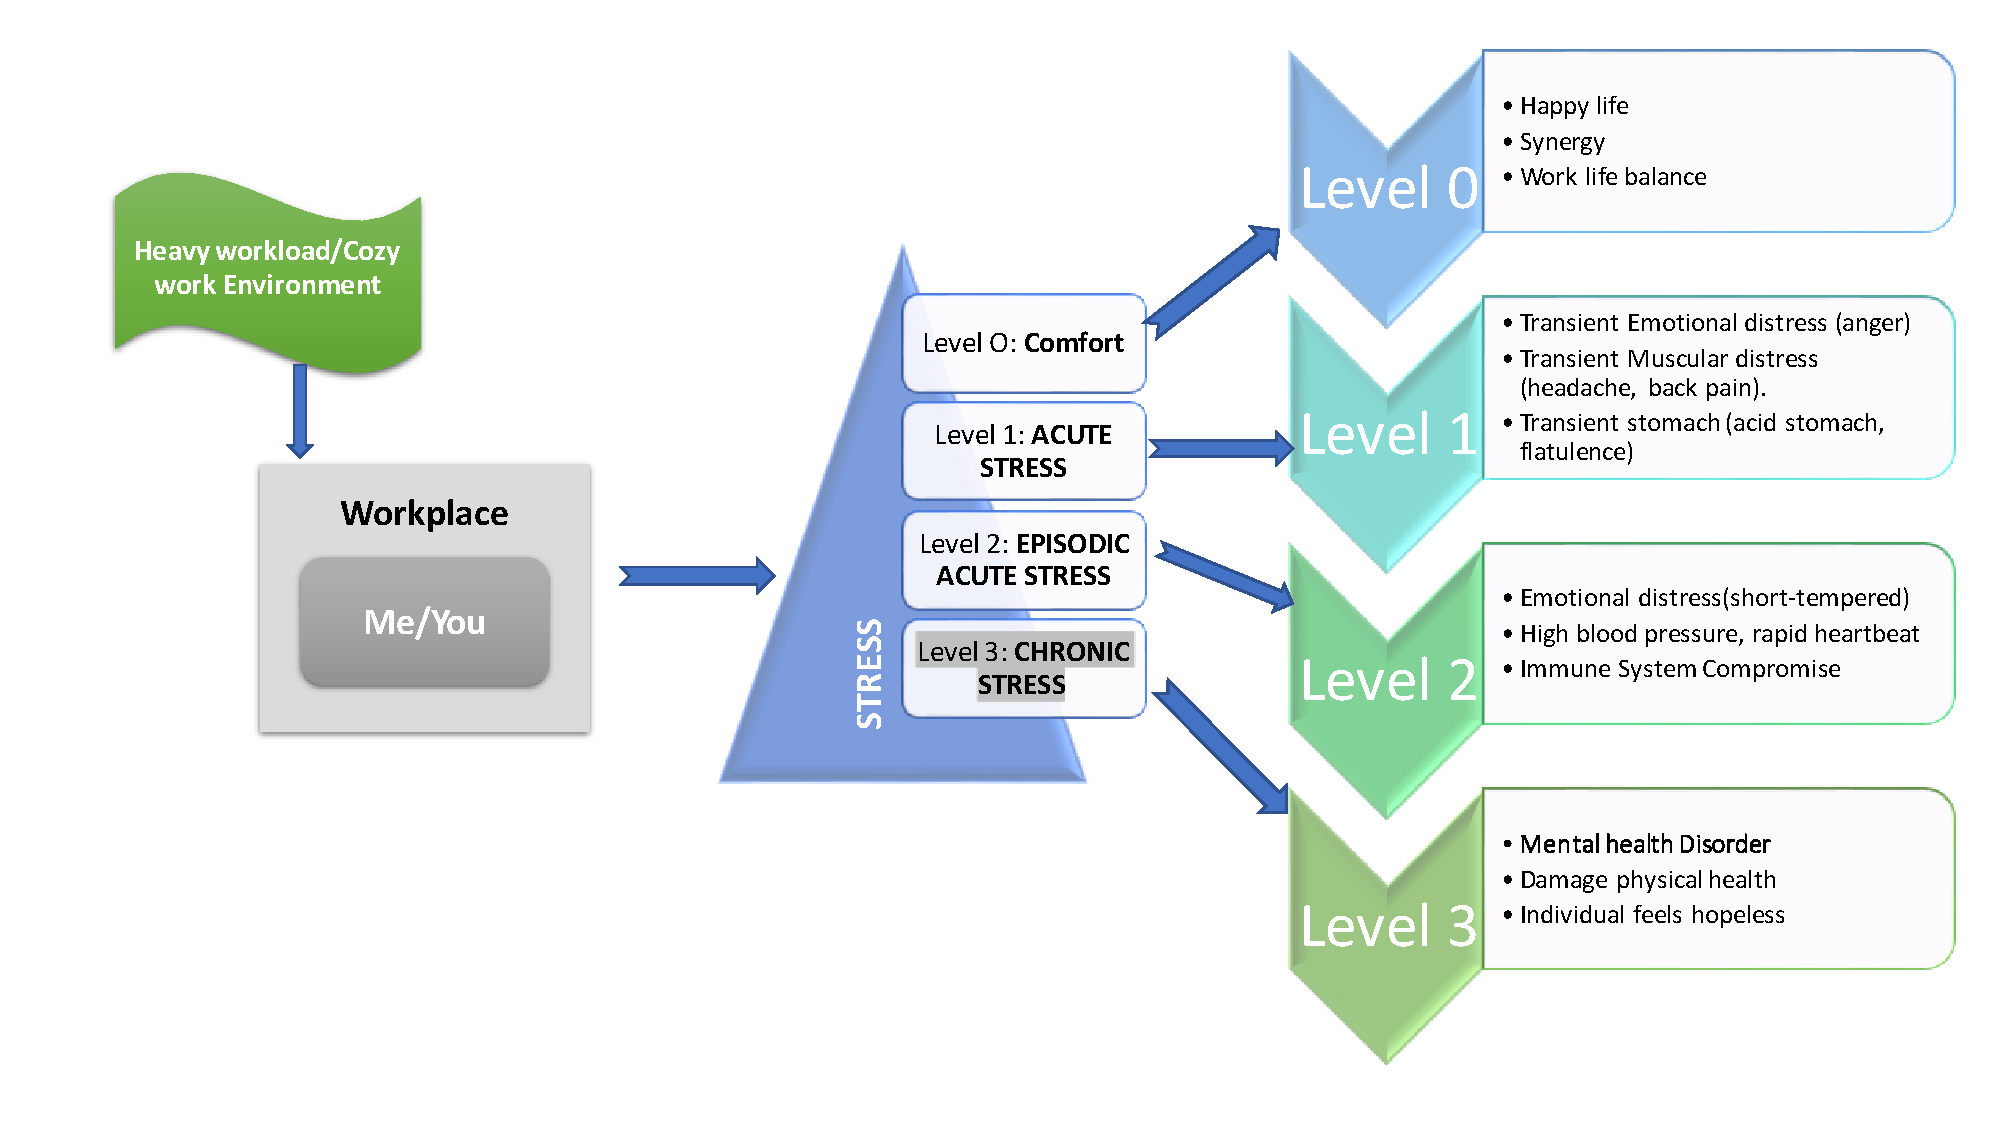
\includegraphics[width=1.10\linewidth]{chap1/images/problem_goal.pdf}
  \caption[Different level of stress ]{Different level of stress with problems.\index{Hasnain}}
  \label{fig:levelOfStress}
\end{figure}

\textbf{Comfort Stress}

Psychologists refer to as "Eustress," is the sort of stress that we feel when we're excited. Our pulse is overeating and our hormones are springing up, but there is no threat or fear. When we ride a roller coaster, compete for a promo, or go on a first date, we feel this type of stress. This good stress has many triggers and it keeps us alive and excited about life.

\textbf{Acute Stress: }

A close call on the street, or speaking before a large crowd, are the kinds of conditions that could cause acute stress. The symptoms are physical, emotional, and/or behavioral but they are usually short-lived.

\textbf{Episodic Acute Stress: }

Episodic acute stress occurs when someone gets frequent bouts of acute stress. People with this kind of stress will oftentimes take on more responsibilities and projects than they can handle. They may seem like they’re constantly in a rush, always running late, and are disorganized. People with episodic acute stress can also be hostile towards others and have strained relationships.

\textbf{Chronic Stress: }

Chronic stress happens when people feel trapped in a bad situation. Whether it's an over-demanding job, an unhappy marriage, or a dire financial situation, this is the kind of stress that starts to wear away a person's physical and mental health significantly.\citep{Cottini2013MentalEurope}

So this section of recognizing stress symptoms should be the first step in understanding whether or not an employee is anxious at the workplace.  Only then can one go to better understand the causes and the letter about better Stress management mechanisms. We now start with personality types or group of people and then types of stressors in order to have a logical flow of hypotheses before we get to the key theories of this study which are causes of stress and stress management.

\section{Disability Group}

\subsection{Types of personality and the degree of being affected by stress} 
A research by Friedman \& Rosenman (1974) established two personality traits they named personalities of type A and type B.  

Type A personalities are prone to stress because of the pressure they put on themselves, they are constantly trying to multi-task, they are violent and nervous. Whereas the personalities of type B are more calm and relaxed.

Due to the hard work type A personalities put into their careers they are more likely to be promoted and have control over their career, but they are also the ones that are likely to be reported to have too much stress or suffer from health issues. And the suffering people with such characteristics never get to the top of corporate hierarchy because of frustration and lack of patience.

While type A personalities are much better in comparison with type B personalities, type B personalities are much stronger and have the potential to become top executives. Consequently, thoughts of a person depend on how he / she perceives a situation as stressful or not.  Mostly it depends on the temperament of a person, and the level of stress encountered is also influenced by the individual characters of individuals. \citep[p.314]{Bloisi2007ManagementBehaviour}

According to \cite{LazarusR.S.Folkman1984StressCoping.} the degree of stress encountered depends on factors such as market awareness which means that people need to know that there is demand. If people try to satisfy their demand, they might be harmed in the event they don't respond appropriately. Firstly, the threatening situation must be of interest to the individual and consequently the consequence of the demand must be unknown. \citep[p.310]{Bloisi2007ManagementBehaviour}

\subsection{Types of stressors}
Below are stressors which affect an employee in the workplace. 

1, Work role: -this happens when the employee is uncertain as to what job he / she should be doing or when the employee has an enormous amount of work to do with such a short amount of time. Stress may also grow as a result of uncertainty.  This situation will probably occur at any form of occupation.

2, Underutilization: -This means that the worker does not have enough work to boost his / her motivation.

3, Responsibility for others:-This increases the level of stress if workers are faced with high responsibility for others.  Those who are in charge of others at the workplace and those higher up the corporate hierarchy are often vulnerable to greater stress because of their co-workers' expectations.

4, Poor working conditions: -these factors also contribute significantly to stress, which include extreme heat, cold, noise and overcrowded. \citep[p.318-319]{Bloisi2007ManagementBehaviour}

\subsection{Job anxiety and employee Relationship}

Firstly, we use below mentioned equation to estimate the relationship between task anxiety and employee, career and workplace characteristics:

\[JA_{i_j} = X_{i_j} \beta+Z_j \gamma+\epsilon_{i_j}\]

Where \(X { I_j}\) refers to employee's personal and job-related characteristics \textit{i } in the workplace \textit{j } and includes age, gender, race, impairment, highest academic qualifications, part-time employment, temporary employment, occupation, supervisory duties, whether individuals perceive themselves to be over-skilled or under-skilled, and whether they perceive themselves to be over-skilled or under-skilled. Workplace level controls \(Z_j\) include sector, workplace size log, area, existence of an appraisal system within the employee's occupation, and workforce composition (female, age, temporary, full-time). They also account for organizational change (reported by the manager), performance-related compensation, team work prevalence and training receipt.  In addition to these more traditional controls, it is also important to include a measure of co-worker anxiety that was not used in previous studies but could capture common unnoticed effects on the workplace and spillover effects among workers, the latter being noted \citep{Cottini2013MentalEurope}.

\section{Causes of stress}
Employees undergo and feel stressed due to a set of different factors and therefore the occupational stress reactions are not a separate thing. \citep[p.8]{Fairbrother2003WorkplaceSatisfaction} Increasingly, the level of stress among employees is changing rapidly due to a variety of reasons such as work exhaustion, overcrowded workplace, generating noisy machine noise and arousing tensions between employees and employers as a result of poor or inadequate decisions.

Stress may emerge from changes that are made in our personal lives.  Personal issues that lead to stress include family issues such as loss of loved ones, financial problems and divorce.  These can be categorized as individual triggers which lead to stress.  On the other hand, stress is also triggered by organizational factors which are those faced by the workers at the workplace.Issues such as task uncertainty; that is not being able to know exactly what we are supposed to do and what others expect of us and also having too much work at hand with too little time to do it can cause stress at the workplace.  Certain organizational stress factors are poor working environments in which the employee is often too busy, where noise, cold or too warm temperatures are present, and in which the office is often filled with people rushing about.  Whereas problems that lead to stress are lack of control, suddenness and uncertainty; position ambiguity in particular is the primary cause of stress at work. \citep[p.350]{Parker2008PersonalityProcess}

Many organizational variables which can be considered stressors often rely on job types and work requirements.  They play an important role with respect to stress issues, for example if the task is high-stressed or not.  High stress jobs are the kinds of jobs that take plenty of time and put the workers under the work pressure. It is also notable that workers frequently suffer from poor working conditions, if the job is carried out in an uncomfortable atmosphere \cite[p.317]{Bloisi2007ManagementBehaviour}

In  order  to  study  in-depth  the  main  reasons  of  stress  or  why  the  employees  feel  stressed specifically at the workplace, we have described some main factors in the next section that often initiates stress.

\subsection{Workplace factors causing stress}

Scholars have identified a large number of occupational life characteristics as being related to stress.  Workers feeling the stress reaction at the workplace are not a new aspect. Spark \& Cooper (1999) reported their research by performing a retrospective survey of 7,099 workers from 13 different businesses and jobs.   They identified a significant statistical assembly between factor in the workplace and negative health symptoms or mental condition disorder such as anxiety, depression and irritation.

For the following reasons employees usually feel stress at their work.
\begin{enumerate}
    \item Work overload
    \item Misuse of power
    \item Inadequate decisions or leader behaviour
    \item overcrowd, noise
\end{enumerate}


Work and job is itself a stressful phenomenon and is therefore related to stress by various aspects (Defrank \& Ivancevich, 1998; Spark \& Cooper, 1999; Taylor et al., 1997). According to Burke (1988), the factors associated with roles in a work environment are Nilsson \& Burke (2000), namely the presence of low-level authority, arbitrary role or conflict over the position. We add that stress is associated with that physical conditions at the workplace including concurrent permanent noise, overcrowding and lack of confidentiality. Leader's or chief's actions can also influence stress level \cite[p.9]{Fairbrother2003WorkplaceSatisfaction}

\subsection{External Factors of stress}

From an individual perspective as well as in the workplace, we explored the causes of stress. There we concentrate on potential stress factors for both staff and organisations. Employees will be directly affected by external stress factors but corporations are often indirectly affected.

According to the Kirkcaldy \& Martin (2000) report, workers have endured tension because of various reasons. There has been primarily tension associated with important issues, including environmental and economic aspects.   Corporate atmosphere and workplace implications of work contentment, corporate commitment and employee behavioral elements are included in the environmental factors.   For example, in hospitals dealing with wound, death and dying on a regular basis remarkable occupational atmosphere for doctors and nurses. \citet[p.10]{Fairbrother2003WorkplaceSatisfaction}

External factors outside employee and organisation's influence are based on political dynamics and economic factors.  Some of the economic consequences for a business that concerns workers are economic risks such as retirement and downsizing. Changes in political situation or economic hardship are out of the reach of workers, therefore the possibility of retirement and downsizing in some way affects employees. \cite[p.320]{Bloisi2007ManagementBehaviour}

Technological advancement is also another external factor which has largely contributed to productivity. This caused a remarkable decline in labor demand on the market which had an impact on job security for the employee. Although familiarizing oneself with new technologies is necessary, it can be considered stressful if it is viewed as difficult or hard to know. New software may cause stress among employees due to technological changes such as computerized systems. Politics is also an important stress factor, in addition to technological changes. Will render the workplace more difficult in situations where there is significant shift in government policy or employee mistrust against government.  \citep[p.309-320]{Bloisi2007ManagementBehaviour}

A study conducted by Rees (1995) and Young \& Cooper (1995) reported that many research findings and adequate knowledge are available in this particular area. Scholars can not directly apply all of their results to all workplaces because the factors in the workplace are not always linked to stress at specific workplaces or, in other words, stress factors are not always stable, consistent and common to a group of occupations. This ranges from environment to environment, work to work or situation to situation but on the team being surveyed the relationship differs between stress and job satisfaction.  \citep[p.  8]{Fairbrother2003WorkplaceSatisfaction}  

Next, we address stress in a specific context of work to see what can cause stress and identify the roots of the problem in one definite environment of employment.
%09.02.20
\subsection{Stress in a specific job context}
Royal Australian Navy performed an internal staff study on what causes a seagoing ship to be stressed out. (Royal Australian Navy 1996).It defined employees as suffering from stress because of the following different reasons. The survey shows that 35\% of employees working on ships and 25.9\% of regularly employed officers are stress associated with their job. They mentioned a few reasons related to their stressful occupation such as limited work environment situation and living conditions on a seagoing ship. As an unpleasant and restricted situation due to working in an isolated community, respondents demonstrated their salient aspects linked to their stressful work, career, and working environment.  Naval officers, on the other hand, are under pressure because of restrictions and strict schedules that shorten their access to regular personal routine and even interrupt the sleeping time.  Gilks \& Buckley (1995) commonly reported that 50\% of officers are shortening their personal duties to gain time for broken sleep.

It relates to our goal of connecting the causes of stress, whereas here the causes are that the working conditions are beyond employee control and have a negative effect on the employee's\cite[p.~10]{Fairbrother2003WorkplaceSatisfaction}.

By reading this section, the reader has grasped an understanding of the potential causes of stress in personal life, in the workplace, as well as the external factors outside employee and organization control.  So now we can continue to see what potential effects, consequences and drawbacks stress can have on workers and on the company as well.

\subsection{Consequences of stress on employees}
Employee stress consequences Episodic stress is characterized as "a pattern of high stress followed by relaxation periods" while chronic stress is defined as "stress caused by the continuous interaction of stressors without relief \citep[p.313]{Bloisi2007ManagementBehaviour}”The consequences of suffering from adverse chronic stress are divided into three categories: physiological, psychological, and behavioral. Some of the signs of physiological stress are blood pressure, high heart rate, and headaches while psychological symptoms are nervousness, unhappiness, and bad tempered ness all of these emotions can result in lack of concentration, indecision, and absenteeism. If individuals can not find solutions to their stressors they may end up feeling depressed, insane, and often refuse to believe in being caught up in an imaginary life. Higher alcohol intake, aggressive attitudes, and restlessness are the behavioral consequences of individuals subject to chronic stress \citep[p.323]{Bloisi2007ManagementBehaviour}

Another consequence of stress is that it can cause a lot of illnesses.  There is evidence that stress may be one of the causes of these diseases; coronary heart disease, hypertension, and cancer, but the degree to which one person is affected by a stress-related disease often greatly depends on what kind of personality that person has, i.e. if that person has type A personality or type B personality.  (Friedman  \&  Rosenman  (1974)  Also  Friedman  \&  Ulmer (1984)describe Type A personalities as competitive, punctual, easily frustrated and perfectionist, whereas Type B individuals are relaxed, sensitive and satisfied with their job and are less prone to stress.

A transition in physiological, psychological, and behavioral improvement could therefore be considered a consequence of stress.  Generally, blood pressure, depression, elevated heart rate etc. are the physiological effects of stress, while the physical consequences are chronic stress causing absenteeism, indecision, nervousness, etc. Sleeping problems, elevated alcohol and smoking habits, frustration, and so on, are the behavioral effects of stress. Confronting the situation is some of the reactions to behavioral stressors. There are two words to be taken into consideration when coping with stress. The first is known as (fight) to address the problem or dilemma and find a solution to it and the second is named (flight) to walk away from the stressors. \citep[p.348]{Parker2008PersonalityProcess}
%10.02.20
\subsection{Disadvantage of stress for employers and employees}
Stress has several adverse effects on the workplace's employee occupational functions. The negative effects include lack of willingness and interest in work, decrease in productivity, reduction in performance, and poor dedication to the company, job and colleagues.  It also increases the level of rigidity and inflexibility related to job performance and provides a space for confusion or disrespect for the organization's laws, policies and regulations. \citep[p.10]{Fairbrother2003WorkplaceSatisfaction} Depending on the management perspective, stress problems can be examined in two ways, stress risks to workers within the company and direct stress impact on the workplace / organization. 

\subsection{Steps towards Stress Management for employees and organizations}
Productive stress management requires three phases for both workers and organisations. 

1, Awareness: it helps to understand when efficiency and absenteeism are declining.

2, Cause determination: Find out what causes this suffering and its effects.

3, Do something constructive: Seek solutions to problems that exist

At one stage tension could be viewed as an unavoidable state. Maintaining productivity complicates the situation and also disturbs having good work and social life. The first step towards stress management is to recognize signs of stress, such as anxiety, frustration, irritation, etc. Upon identifying these symptoms, the next step is to find out the causes and work out their impacts. The third and final step is handling a stressful situation effectively.

There are two types of coping mechanisms proposed by Folkman and Lazarus (1988) the first is that the stressors are either modified or completely removed (problem focused) here. The second mechanism is (emotion-focused) where workers learn to adapt to circumstances, and also cope constructively with stress.  The difference lies in where the stressor is specifically confronted in problem-focused coping mechanism; it is either changed or eliminated. Whereas in emotion-focused it is only the people who change or learn to adapt productively to the stressor. \citep[p.326]{Bloisi2007ManagementBehaviour}

The first person in control (charge) of managing stress eventually rests on the employee and the following are some of the techniques to cope with stress in relation to the workplace.

1, Time management: plan tasks accordingly, efficiently managing one's time, prioritizing tasks to be dealt with first. Efficiency and efficiency are respected here.

2, seeking help: Staff, co-workersor supervisors are encouraged to receive assistance to improve the performance.

3, Emotion-focused strategies: as discussed previously, it is important to learn how to respond to stressors in a positive way. Popular approaches based on emotion include exercise, companionship, relaxation and leisure activities. \citep[p.328-333]{Bloisi2007ManagementBehaviour}

\section{Employees stress management at the workplace using Smart \acs{IoT}}
In most situations, the staff and organizational strategies try to reduce the threat to the health of workers in their workplace associated with stress.  Specific strategies involve many methods, such as workplace, physical and psychological seminars, routine instruction, consulting counselors, etc., to reduce the risk of stress associated with employee health. The exact purpose of these consultations and activities is helpful in helping workers become aware of the available resources.

Existing services and tools help employees improve their skills and abilities against challenging circumstances, or alter their current situations. (E.g. physical, psychological, occupational). A wide variety of training courses are offered to help employees improve their skills.  (e.g. effective or sufficient management, time management, communication skills, assertiveness, problem-solving etc.). Both behaviors lead to higher work performance and positive employee performance toward stress and coping with it. 

Training helps workers illustrate the following features:
\begin{itemize}
    \item One can understand the signs of stress 
    \item Gains versatility in behavioral patterns, and when it begins, one can participate in the stress cycle. In a typical situation tension usually grows slowly. More tension brings more trouble. 
    \item It allows situational awareness and offers a plan of action to reduce stressors.
    \item Develop ways of effectively reacting to stress and the correct coping mechanisms. 
    \item Learn coping skills, motivation skills, and improved self-confidence.
\end{itemize}

The above methods have proven helpful in managing stress or in preventing increasing stress. (Michie, 2002, p.69-70)

\subsection{Smart \acs{IoT} for Stress management}
%need Rephraise
Over the past few years, \acs{IoT} technologies have been widely applied in various health fields through many initiatives. \acs{IoT}-based devices, such as mobile phones and wearable computing, are often used in the field of health metric self-measurement.  These tests are used to promote health, well-being and stress management where improvements in critical parameters can be observed and play a role in changing human behaviour. 

Various types of wearable and sensors used individually and in combination, are designed to track vital parameters that indicate stress or arousal symptoms, such as heart rate, GSR (galvanic skin response), blood pressure, and others. 

Heart rate is one of the markers of health status, a reflection of the presence of anticipation.  Heart rate monitor is commonly used in sports equipment\citep{Fu2015SystemDevice} and fitness.  The heart rate sensor will boost the detection of stress levels in daily life and help to provide stress management\cite[p.330-339]{Millings2015CanTechnology} \cite[p.361-371]{Parnandi2017PhysiologicalGames}.

Smartphones play a large part in managing stress.  Some apps have embedded sensors to detect and track stress-or depression-indicating behaviors\cite[p.175]{Saeb2015MobileStudy}. Others introduced biofeedback, i.e. stress and anxiety therapies\cite[p.1274-1286]{AlOsman2016UbiquitousManagement}\citep{Zafar2017PlayingBiofeedback}. Ahtinen proposed a mobile stress management application that includes four mental wellness-training intervention modules\cite[p.11]{Ahtinen2013MobileStudy}. The study, which recruited 15 university participants, has shown significant improvements in respondents ' stress and life satisfaction.

One consumer stress management system is Biosync Technology. The heart rate of the patient, the galvanic reaction to the skin and the gestures are measured. Data are processed automatically to assess the stress level of the patient and, in turn, preventive measures are given to ensure a better life\citep{Nishida2017BioSync:Experience}.

A number of papers investigated the assessment of the psychological condition and physical reactions in students\citep{Santos-Gago2019InnovativeReview} and their academic success, as well as the estimation of their correlation, or the improvement of the mental health of students. Shen, Wang \& Shen's research \citep{article} used psychological cues to predict emotions.  In the research cycle they explored the existence of different emotions and suggested a sensible e-learning model. The data were collected using three sensors: the skin conductivity sensor measuring electrodermal activity, the blood pressure measuring photoplethysmograph sensor and the brain activity measuring EEG sensor. In the natural environment, measurements were taken over several weeks on one subject, as close as possible to the daily environment.

In this research we want to design and implement a system to identify the psycho-physiological signals that signify stress in the workplace during work. Some research uses different types of devices to understand occupational tension, but few of them cope in a real environment with stress management. Our goal is to provide a solution that would validate stress feeling and help employees manage their stress during work.

A mobile application with the relaxation material will reduce employee anticipation and have an effect on stress reduction during work.
\section{Summary of Related Work theories}
To sum up the theoretical chapter and the core theories discussed in this section, stress, causes of stress and the management of stress with each core theory including subtopics such as symptoms of stress, personality types, factors of stress, workplace factors causing stress, types of stressors, consequences and disadvantages of stress on employees and organizations, employees stress management and organizational approaches to stress management were discussed.
%10.02.20 evening

This chapter tarted off with the presentation of what stress is and the definitions provided on this subject by various scholars.  Some of the stress symptoms were addressed with a view to defining a condition as stressful. Our research seeks to explain why and how stress is handled. We addressed the various causes of stress, because the probability of being affected or the likelihood of perceiving a situation as stressful depends largely on the individual's personality. Further the disadvantages and consequences of stress have been described for employees and the organization in order to achieve productive stress management.

To have an effective stress management system one should be able to know the causes of stress and how it will affect the workers, and then address its implications.  Therefore, after looking at the effects and causes in the workplace, we saw the strategies used to minimize the negative impact of stress from both the viewpoint of the workers and the management of human resources.

The theories chosen are important to our intent, because they were chosen from the beginning to tackle the stress problem that starts from defining what stress is. In doing so, it clarifies what we are going to be talking about to readers from the start and the reader wouldn't have to turn to other sources to understand the concepts by our paper as they've been clearly stated and clarified enough.  The theory of causes of stress is important for our research to understand whether the causes of stress are linked to personal or work. This fulfills our goal of recognizing what causes stress in both employees and management. Since recognizing the causes of stress, we decided to find out how to manage stress from the viewpoint of both the employee and the management.

The inference in relation to our intent which can be drawn from the hypotheses is that the causes of stress in the workplace are job fatigue, poor working conditions such as overcrowded working conditions and noise.  And the stress of Employee can be managed through proper time management, seeking help from \acs{HRM}. The emotion concentrated on activities such as recreation, companionship, and exercise. Management plays an important role in determining and controlling the stress level of workers in the workplace and should use various methods to reduce stress such as implementing training courses to assist the skills of the employee, providing a better working environment and ensuring that employees receive adequate feedback and advice when necessary. The description is the method we will be evaluating the data from.

Now that the reader has an understanding of what stress is and why we find this topic fascinating we would now like to go on to the next chapter that is the design chapter, discusses how we perform requirement engineering and persona analysis for this report.
    \chapter{Concept}
\textit{In  this  chapter  we  will  discuss about concept  that  address  the  topics  of  stress management requirement engineering and design approach .  We  have  chosen requirement engineering  that  assisted  us  to design a system for stress management at  the  workplace  in  particular  for people with stress disorder.  To  have  a  clear understanding of the requirement we have chosen the design process.  It organize our ideas and refine potential solutions to engineering challenges. Afterwards  a  system is designed which is satisfy our goal.}
\vspace{5mm}

Stress has recently overtaken the common cold as the most common cause of sick leave in many European countries and is a major cause of concern for companies worldwide. Why then do most of the 'Coping with Stress' texts to be found in bookshops consider this a problem only to be tackled by the Individual ? Strategic Stress Management is different, it shows how companies can boost performance by adopting integrated organizational strategies to identify and reduce stress in their employees. Including practical advice on how to conduct a stress audit and how to target stress 'hot spots' with an organization, Strategic Stress Management provides a fresh strategic model for the manager concerned with the negative effects stress can have both on company performance and the quality of life of individuals at work. This is the latest book from best-selling stress management author, Cary Cooper, and will be eagerly awaited by HR Directors, Organizational Consultants. Occupational Psychologists, Managing Directors and all managers who wish to work with healthy, stable and productive staff.

\section{Requirement Engineering}
The ultimate aim of writing a problem statement is to turn a common problem into a targeted, well-defined problem that can be solved through a requirement engineering process. It clearly indicates the project's purpose. \citep{K.AduMichael2014InadequateStudy.}

\begin{figure}[ht!]
\centering
\smartdiagramset{
planet color=orange!60,
distance planet-satellite=4cm,
planet text width=2.5cm,
satellite text width=2.7cm,
}
\smartdiagram[connected constellation diagram]{
    Requirement Engineering,
    Feasibility\\study,
    Analysis,
    Definition,
    Documentation
}
\captionof{figure}{Requirement Engineering Steps}
  \label{fig:RE}
\end{figure}

It is a process of gathering and defining service provided by the system. Our requirements Engineering Process consists of the following main activities: shows in figure:\ref{fig:RE}

\begin{enumerate}
    \item  Feasibility study : find out the current user need and budget.
    \item Requirement analysis: what the stakeholders required from the system.
    \item Requirement definition: defined the requirements in the form of understandable to the customer.
    \item Requirement document: official statement define both, definition and specification.
\end{enumerate}

The current research aimed to explore the effectiveness of a system that promotes behavioural change for stress-related issues in terms of the acceptability, usefulness, and possible effects of the program. Furthermore, the aim was also to study how appropriate and realistic the process and resource management of the study would be for a randomized controlled trial. \citep{Eklund2018EvaluationStudy}

When conducting a feasibility investigation, the important parameters for a planned, randomized controlled trial can be identified, adjusted, and further developed to improve the chances of success in a larger, more costly study. Feasibility studies can help identify what needs to be changed in terms of action and research methodology

We taken in person interview for conducting feasibility study based on random set of questionnaires.Following table:\ref{tab:feasibility} describe the result of our interview. 

\begin{table}[ht!]
\centering
\begin{tabular}{|l|l|}
\hline
\textbf{Questions} & \textbf{Answers} \\ 
\hline
Do you feel stress in Working Place? & Yes \\ 
\hline
\begin{tabular}[c]{@{}l@{}}Can you describe a time when your \\ stress resulted in making errors at work?\end{tabular} & Evening \\ \hline
What are the signs of your stress in the workplace? & Can not communicate with others  \\ \hline
How common is stress in the workplace? & Almost Everyday \\ \hline
\begin{tabular}[c]{@{}l@{}}What’s the most stressful situation \\ you’ve faced at work so far? How did you handle it?\end{tabular} & In meeting \& leave the place \\ \hline
When you feel stress what happened in physically?? & Feeling imbalanced  \\ \hline
\end{tabular}
\caption{Feasibility Study Questionnaires \& Answers }
\label{tab:feasibility}
\end{table}

Considering the program's acceptability, the findings for the statements evaluating the opinions and experiences of the participants with regard to the content, tailoring, input, performing an own behavioral analysis, setting goals, graphic and pedagogical design, and how the knowledge is summarized in Table: \ref{tab:feasibility}

To enhance flexibility, participants suggested stress Management should be delivered as a mobile application. Stress Management structure forces user to go through all the assignments in a predetermined order, and this was perceived as a barrier for using. The participant with low stress levels expressed that for a person with a low stress level, it was difficult to stay motivated to go through such an extensive program.In the next section we are going to develop a design approach.

\section{Design Approach}
Providing access to this original information about users will enable agile, progressive, or iterative progress along the development process. In this regard, personas, which are commonly used in user-centered design and human-computer interaction activities, are not only a suitable method for the adequate documentation of users’ attributes, but also a tool for empathizing with users’ aims and needs. Personas can be used throughout the entire development process and in addition to user-centric design tasks by the development team for requirement engineering activities.

The integration of personas, as a kind of user description, in the requirements engineering activities, improves two aspects of the development: (1) consideration of multi-faceted user needs in the early stages of development when practical main decisions are taken; (2) continuous integration, testing and revision of user requirements for evaluation of existing prototypes and intermediates.\citep{Mayas2016PersonasChallenges}

\subsection{Persona analysis}
% https://app.milanote.com/1IW8dZ1W4EN68B/jan
\begin{figure}[hbt!] 
  \centering
  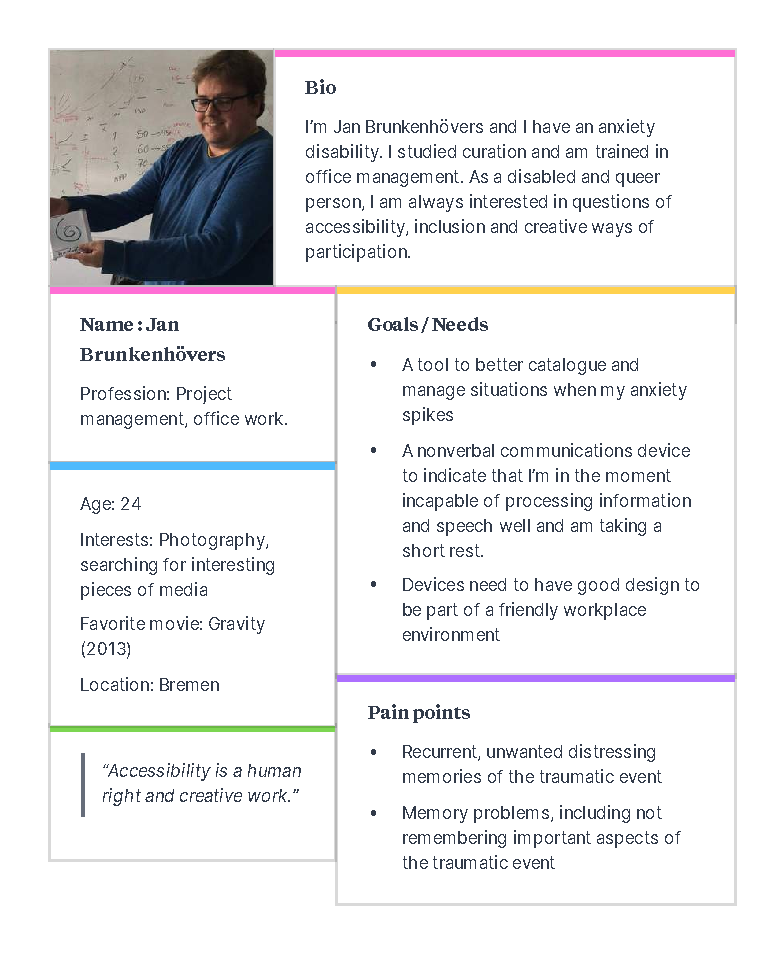
\includegraphics[width=1.05\linewidth]{chap3/image/persona_jans.pdf}
  \caption[Persona Analysis ]{Persona Analysis.\index{Hasnain}}
  \label{fig:Persona_Analysis}
\end{figure}


In Figure \ref{fig:Persona_Analysis} you can see the persona analysis dashboard which has made for the design more specific application for user.

The result of Persona Analysis will be determine based on following data from user:

\begin{itemize}
    \item User Name : Jan Brunkenhövers
    \item Audience segment: Workplace accessibility for anxiety related disability
\end{itemize}
\textbf{Bio}

    "I’m Jan Brunkenhövers and I have an anxiety disability. I studied curation and am trained in office management. As a disabled and queer person, I am always interested in questions of accessibility, inclusion and creative ways of participation."\\
    
\textbf{Personal Information}
\begin{itemize}
\item Age: not mentioned
\item male
\item Interests: Photography, searching for interesting pieces of media.
\item Favorite movie: Gravity (2013)
\item Location: Bremen 
\end{itemize}
\textbf{Goals and Needs}
\begin{itemize}
    \item A tool to better catalogue and manage situations when my anxiety spikes
    \item A nonverbal communications device to indicate that I’m in the moment incapable of processing information and speech well and am taking a short rest.
    \item Devices need to have good design to be part of a friendly workplace environment   
\end{itemize}
% https://app.milanote.com/1IW8dZ1W4EN68B/jan
\begin{figure}[hbt!] 
  \centering
  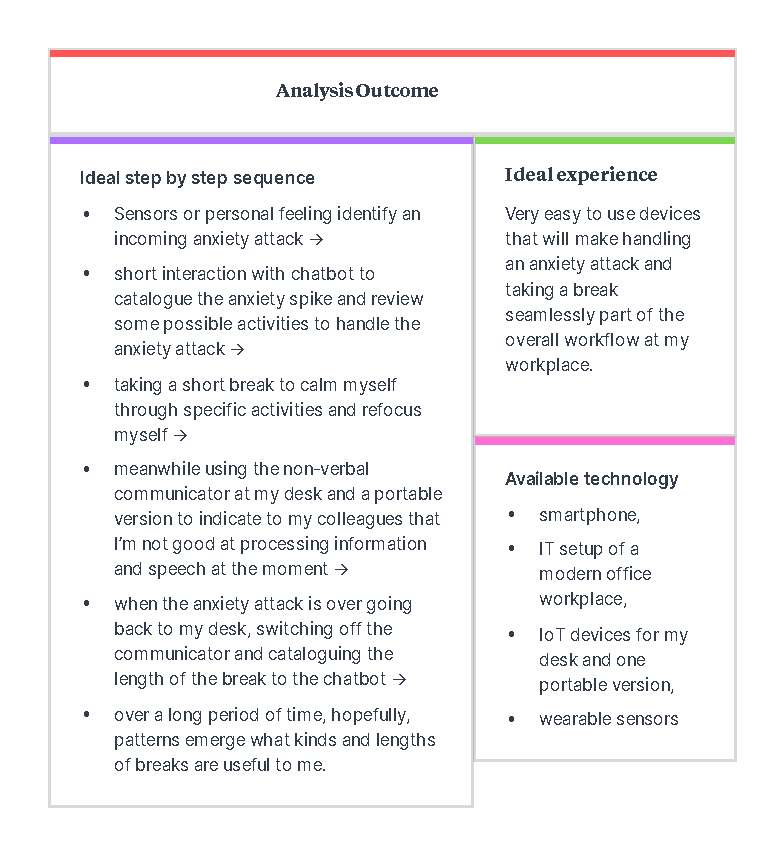
\includegraphics[width=1.05\linewidth]{chap3/image/persona_jans2.pdf}
  \caption[Persona Analysis outcome ]{Persona Analysis Outcome.\index{Hasnain}}
  \label{fig:Persona_Analysis2}
\end{figure}

\textbf{Pain points}
\begin{itemize}
    \item Recurrent, unwanted distressing memories of the traumatic event
    \item Memory problems, including not remembering important aspects of the traumatic event
\end{itemize}

\subsubsection{Analysis Outcome}

\textbf{Ideal step by step sequence}
\begin{itemize}
    \item Sensors or personal feeling identify an incoming anxiety attack 
    \item short interaction with chatbot to catalogue the anxiety spike and review some possible activities to handle the anxiety attack 
    \item taking a short break to calm myself through specific activities and refocus myself 
    \item meanwhile using the non-verbal communicator at my desk and a portable version to indicate to my colleagues that I’m not good at processing information and speech at the moment 
    \item when the anxiety attack is over going back to my desk, switching off the communicator and cataloguing the length of the break to the chatbot 
    \item over a long period of time, hopefully, patterns emerge what kinds and lengths of breaks are useful to me.
\end{itemize}
\textbf{Available technology}
\begin{itemize}
    \item Smartphone
    \item IT setup of a modern office workplace
    \item IoT devices for my desk and one portable version
    \item wearable sensors
    \item Web applications and software's.
\end{itemize}
\textbf{Ideal experience}

Jan said his experience after analysis "Very easy to use devices that will make handling an anxiety attack and taking a break seamlessly part of the overall workflow at my workplace."

based on persona analysis we designed and make a prototype of the application which explain in next section.

\subsection{Use case-driven system block diagram}
In figure \ref{fig:system_block}, We generate a system block diagram to approach it from implementation cases that we receive from persona analysis. This system block diagram is a high-level system modularization that divides the system as a whole into maximally decoupled sub-systems. It helps one to imagine the system as large interacting components, which can be independently conceptualized and created.
\begin{figure}[h] 
  \centering
  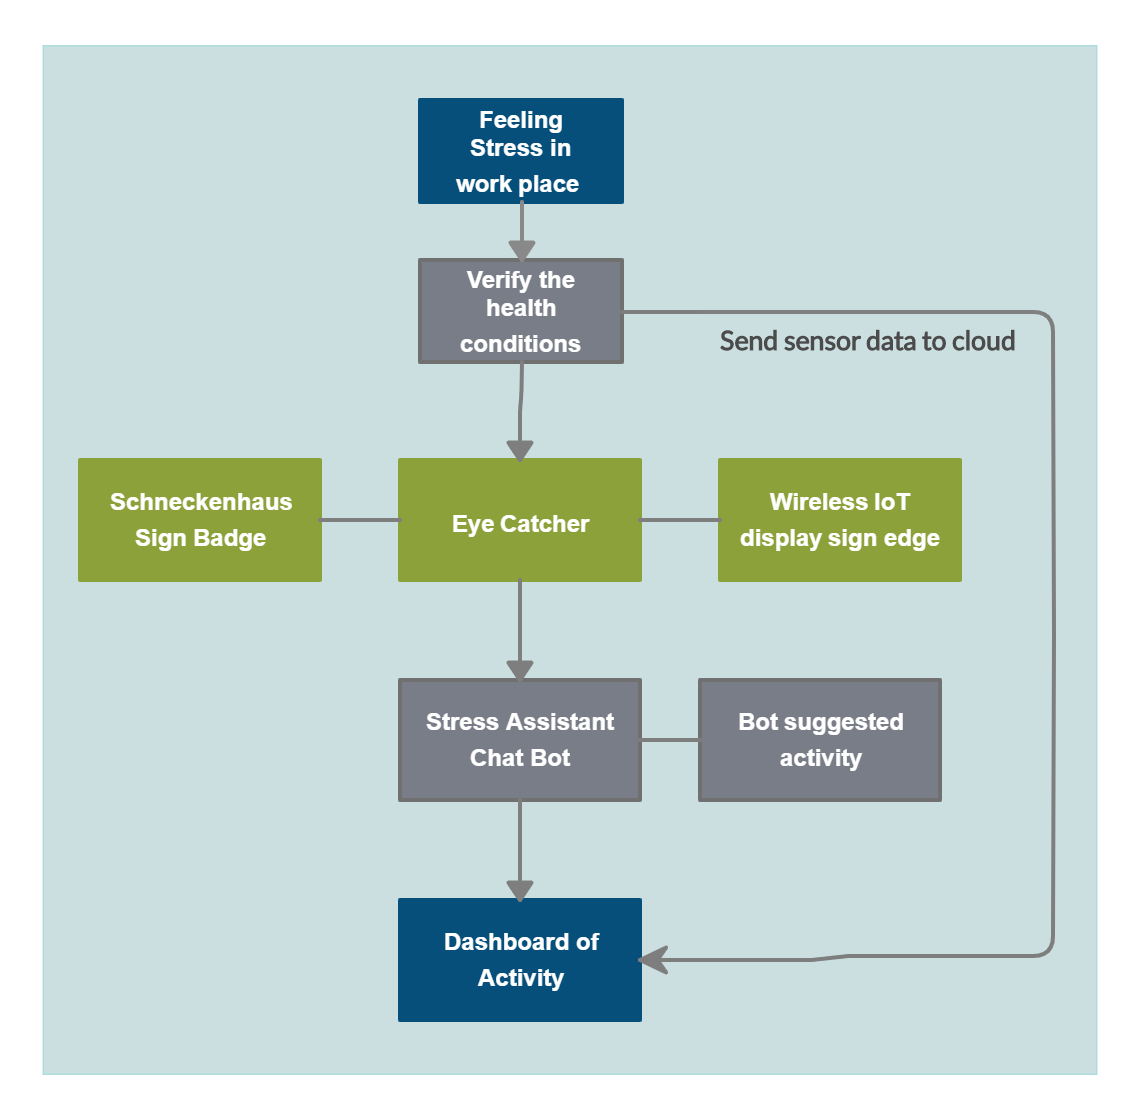
\includegraphics[width=1\textwidth]{chap4/block1.png} %https://app.creately.com/diagram/FLSbOaB2Ejl/edit
  \caption[Stress management System Block Diagram]{Stress management System Block Diagram \index{Hasnain}}
  \label{fig:system_block}
\end{figure}

\section{Prototyping of the Application}

After the persona analysis and block diagram of the application , prior to start implementing and developing it , prototyping has been used as the first step in the design process.

Prototyping is not just about designing a user interface's "feel." It's also about prototyping — deciding how the \acs{UI} should work, and reacting to user input. That is why the design of interaction and the use of cases function together so well, especially when combined with people.\citep{Stephens2006PersonaAnalysis}

\subsection{Paper Prototyping}

\begin{figure}[hbt!] 
  \centering
  \subbottom[Sketch welcome page]{
\includegraphics[width=0.45\textwidth]{chap3/image/sk1.jpg}}\qquad
    \subbottom[Sketch Options]{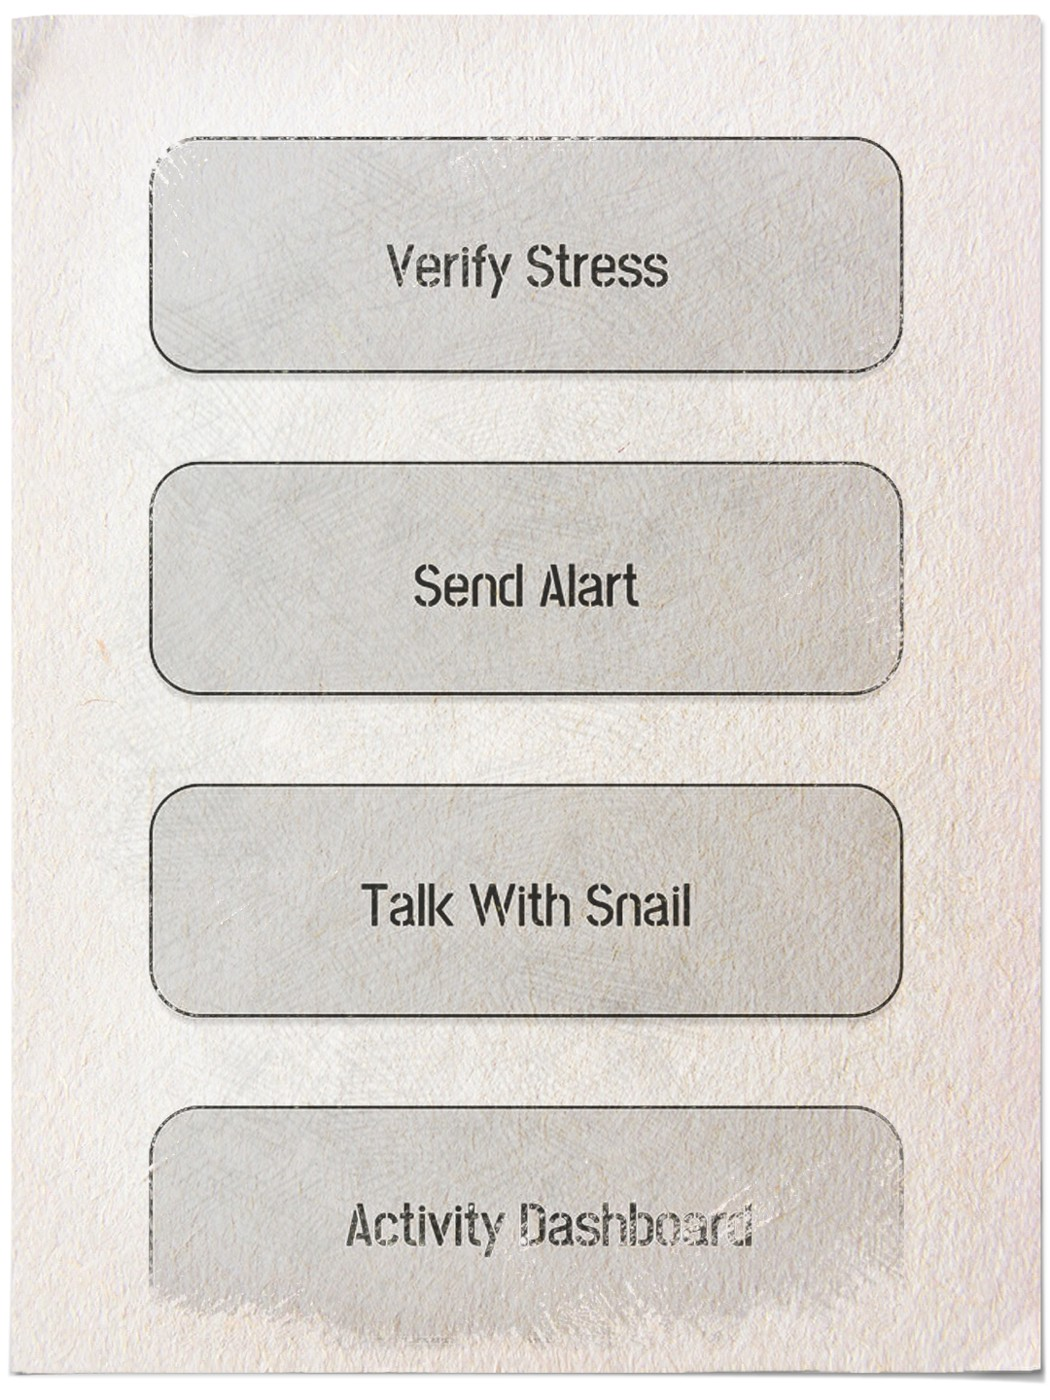
\includegraphics[width=0.45\textwidth]{chap3/image/sk2.jpg}}%
  \caption[Paper prototype sketch ]{Paper prototype sketch .\index{Hasnain}}
  \label{fig:Paper_proto}
\end{figure}
Paper prototyping which is also called as offline prototyping is the fastest way to get the straight feedback from the user in the initial stages of design process and it also makes the discussion easier between the developers and other stakeholders of the app. The easiest ways to create paper prototypes include the use of cardboard, paper, pens and sticky notes.\citep{Bansemir2014ExperienceVisualizations}

The sketches made in paper prototypes create a mutual understanding of the interface of the application between the different stakeholders of the app which further positively affects the development process. It is being said that user and developers find sketches easier to understand the lengthy written documentation. Sketches which are being used in the process of paper prototyping presents the initial ideas of the app and build the foundation of discussions for the further iteration stages\citep{Bansemir2014ExperienceVisualizations}.

In Figure \ref{fig:Paper_proto} and , you can see an example of the sketch which has been made for first look of workplace stress management app.This screen is normally referred to as virtual accessibility assistance or welcome screen. you can see rough sketch of the buttons which we have used for accessing different functionality. 

One of the great things about paper prototypes is the way we come up with all kinds of creative ways of simulating visual effects or interactions.

We plan to conduct testing sessions with a paper prototype and use two roles for each testing session:
\begin{itemize}
    \item Facilitator (presenter). A person who instructs and interacts with the test participants.
    \item 'Human computer' This person remains silent during the session and is responsible for changing screens or screen statements whenever the participant of the test interacts with a prototype.
\end{itemize}

In Figure \ref{fig:Poster}, you can see an example of the testing sessions with a paper prototype which has been made for simulating visual effects of workplace stress management app.We also give a name "Schneckenhaus" to this system.

\begin{figure}[hbt!] 
  \centering
  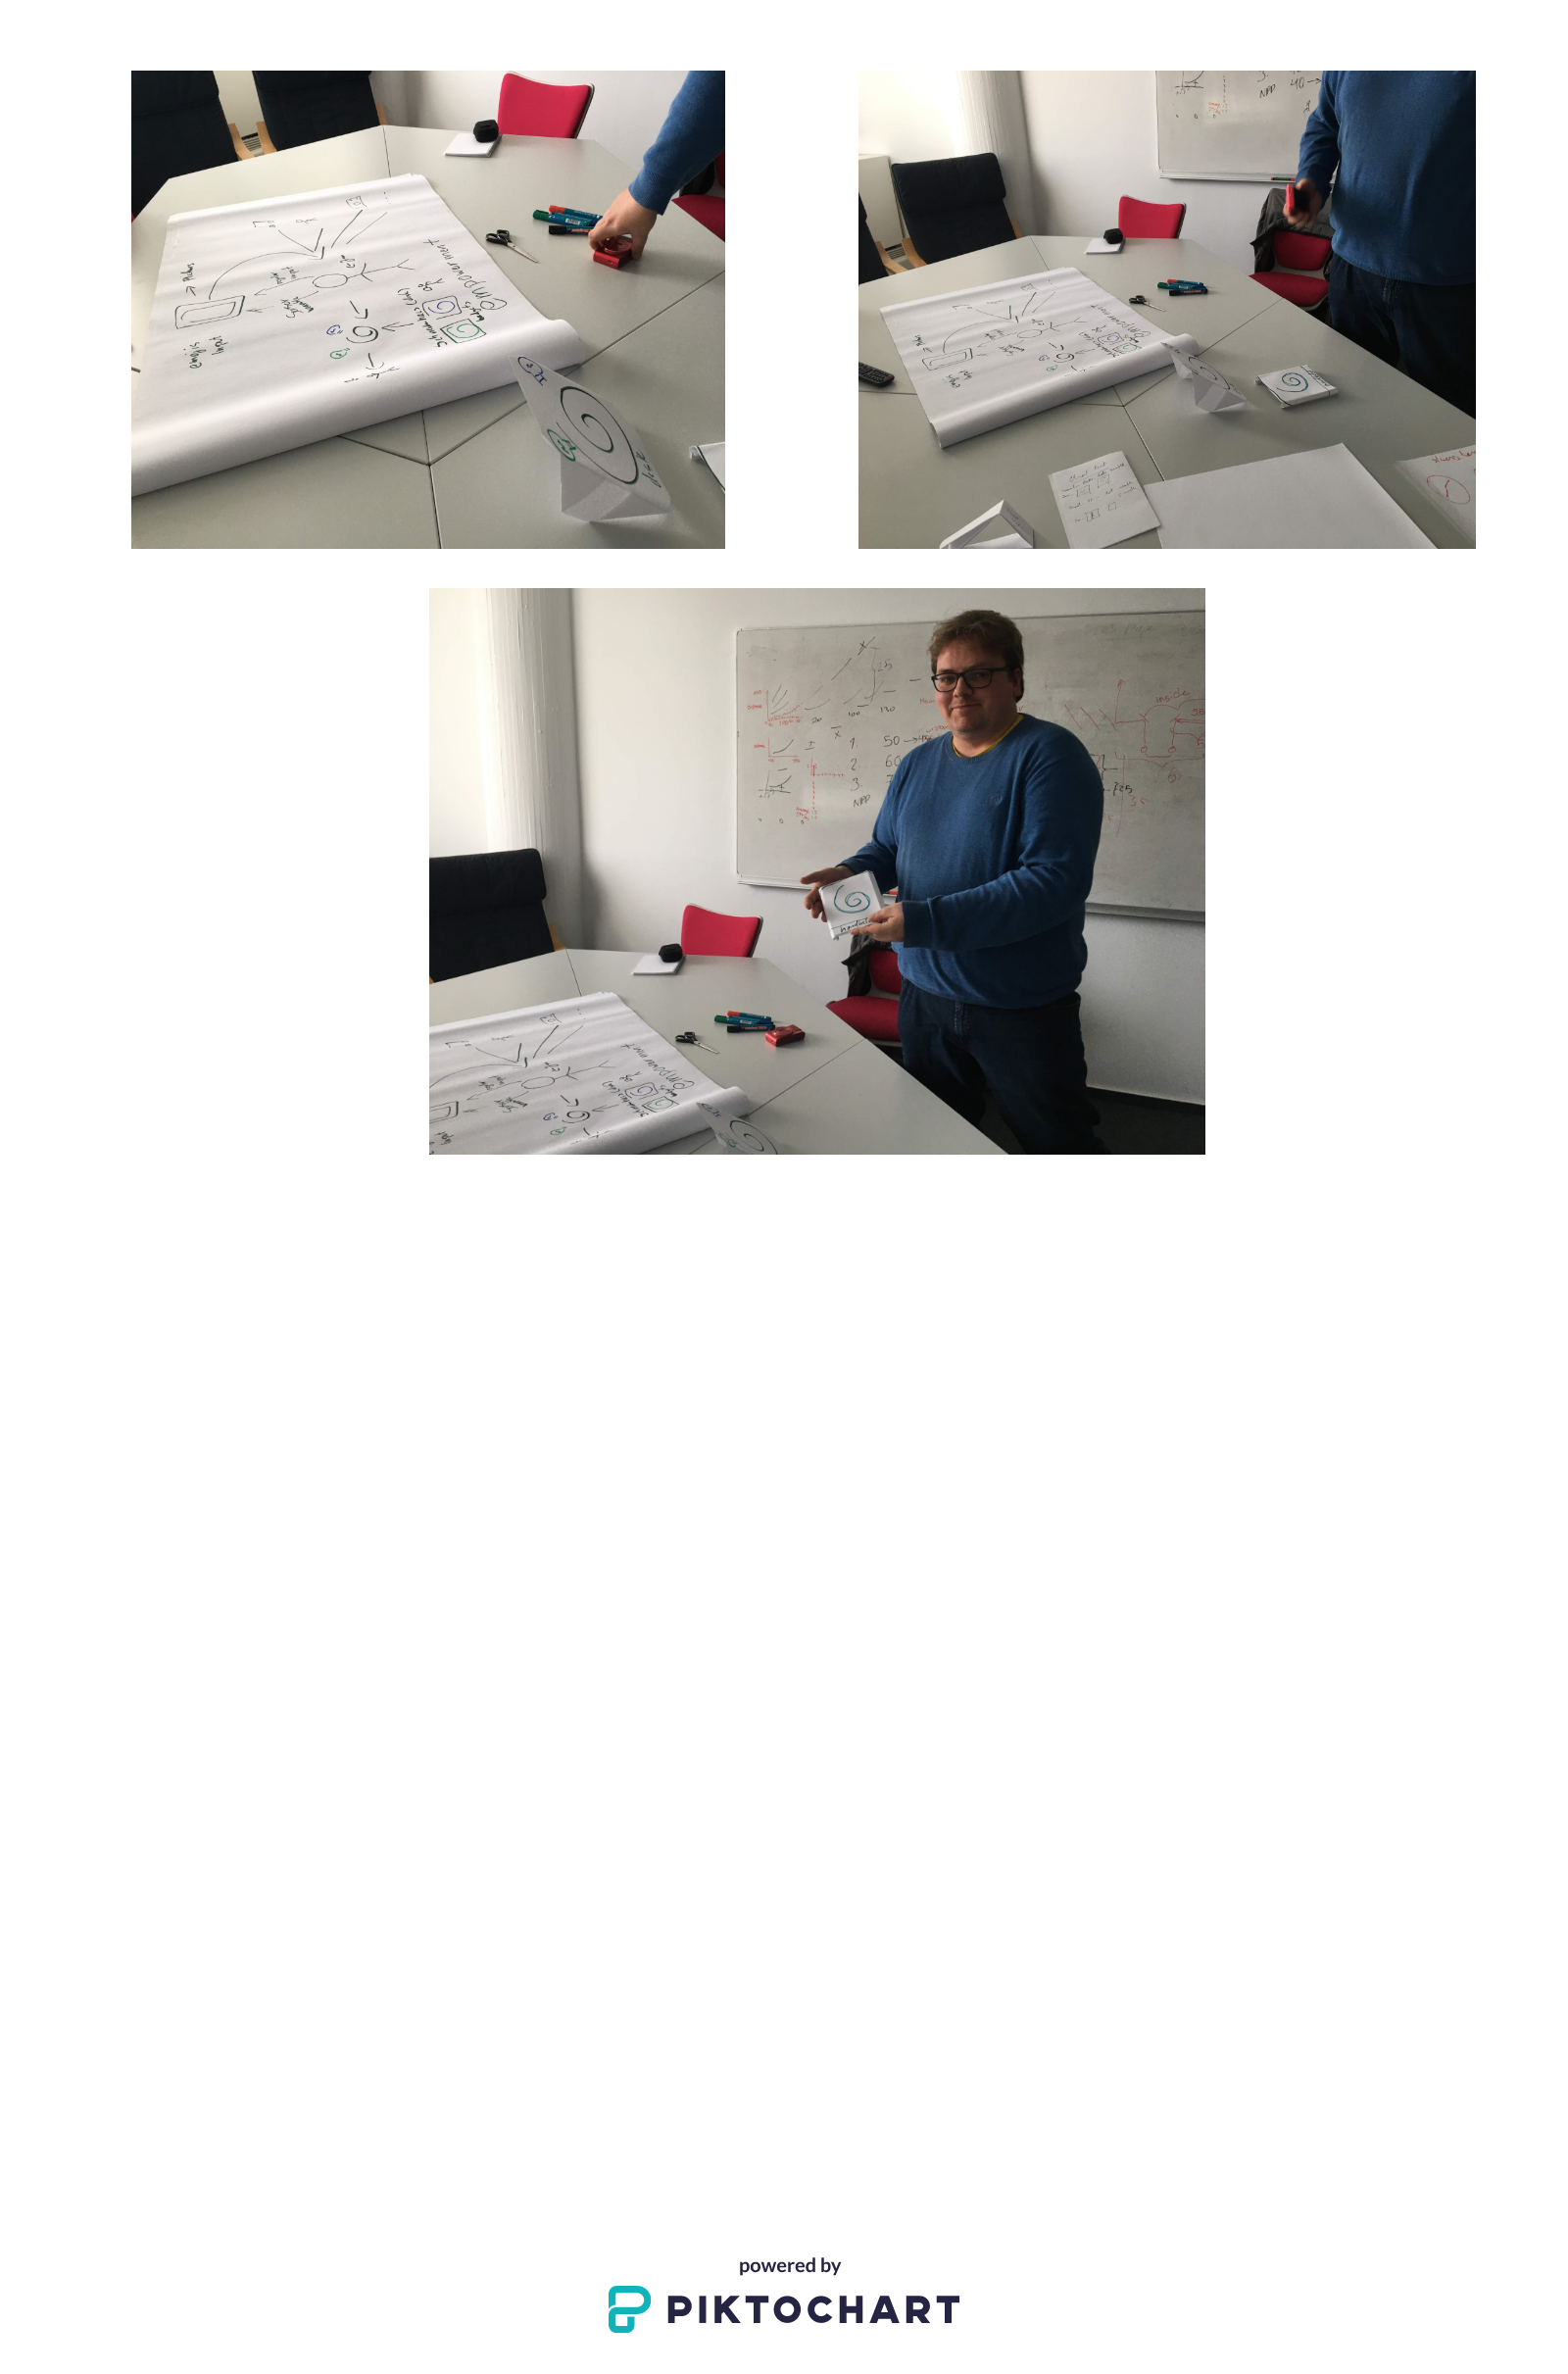
\includegraphics[width=0.9\textwidth]{chap3/image/poster.png}
  \caption[Paper prototype Test ]{Paper prototype Test .\index{Hasnain}}
  \label{fig:Poster}
\end{figure}

The screenshots of the application which has been planned in the prototyping phase and later designed in the implementation phase can be seen in Appendix A.


To sum up; this chapter has discussed the concept and prototyping chosen for performing this study. We have addressed the requirement engineering and persona analysis considerations and also gave reasons as to why we  chose  the  concept  that  we have  chosen. The next section of our paper will then present our system development which we got from the analysis. 


%\enlargethispage{\baselineskip} % so you do not get a single line in another page
    \chapter{The Schneckenhaus System}
\textit{In this chapter, I will address the topics of stress management system (Schneckenhaus) development. Discusses the development of the system and all elements which I have been used to implement the system for stress management at the  workplace  in  particular  for people with stress overflow}
\vspace{5mm}

A stress management system named \textbf{Schneckenhaus} has been developed to achieve the aim and objective of the research which is to decrease the stress level and empower the users through this system. 

Feeling stressed most of the time in the workplace which I have focused on in the initial phase of the thesis is a stress overflow. An extensive literature review has been done in chapter 2: Related work to get ourselves aware of the problem in detail before we started developing the system.

The main goal of developing this system is to create a user's friendly stress management system that can manage stress when they overflowed. In the next section of this chapter, I will explain details about the Schneckenhaus system design.

\section{System Design}
System design is the process of designing the elements of a system such as the architecture, modules and devices, the different interfaces of those components and the data flowing through that system. 

The aim of the system design process in my thesis is to provide sufficient detailed data and information about the system, and this system elements to allow implementation consistent with the architectural entities as described in system architecture models and views.

Making system design more specific firstly I design \acf{UX} and then I develop \acf{UI}.
\subsection*{\acf{UX}}
Designing user experience is a human-first process of product design. A cognitive scientist and co-founder of the Nielsen Norman Group Design Consultancy, Don Norman has been credited with coining the term "user experience" in the late 1990s. He defines it this way:

    \say{User experience encompasses all aspects of the end-users interaction with the company, its services, and its products.}
– Don Norman, Cognitive Scientist \& User Experience Architect \citep{Norman1988TheThings}

I use persona analysis outcome (mentioned in section:\ref{Persona Analysis Outcome}) and paper prototype findings (mentioned in section:\ref{Findings of Paper prototype}) to design \acf{UX}  for our stress management system \textbf{Schneckenhaus}. 

\subsubsection*{User Experience Design Process}
User experience design process is an iterative method that helps me continuously improve and polish my designs. In the process, I go through different stages repeatedly while evaluating my designs on each stage. Each stage involves relevant stakeholders in my thesis that take part in the process to make my thesis highly efficient and usable.

Schneckenhaus system UX design process involves following six stages based on: \citep{Minhas2018UserPlanet}

\begin{itemize}
    \item \textbf{Understand:} Understand requirements create user personas define use case.
    \item \textbf{Research:} Analyze related work research latest UX trends
    \item \textbf{Sketch:} Gather ideas draw sketches and wireframes evaluate and re-draw
    \item \textbf{Design:} Design Images, Create prototypes, Define UX guidelines
    \item \textbf{Implement:} Implement functionally build experience
    \item \textbf{Evaluate:} Perform usability testing, identify improvements.
\end{itemize}

Considering \acf{UX} In the next section we will discuss about \acf{UI} development.

\subsection*{\acf{UI}}
Schneckenhaus system UI is being developed in the android platform using the latest coding language, standards, and practices of Android Programming. The programming language which has been used to develop this app is Kotlin. 

According to Kotlin's official website "Kotlin is a cross-platform, statically typed, general-purpose programming language with type inference. Kotlin is designed to interoperate fully with Java, and the JVM (Java Virtual  Machine) version. 'In Google I / O 2017, Google officially supported Kotlin for mobile development in Android. And the company also encouraged Android Developers to start developing their apps in Kotlin. 

For making the system more user-friendly, I developed a single app solution and integrate all functionality of the Schneckenhaus system. In the next section, I will discuss the system overview.

\section{System Overview}

\begin{figure}[hbt!] 
  \centering
  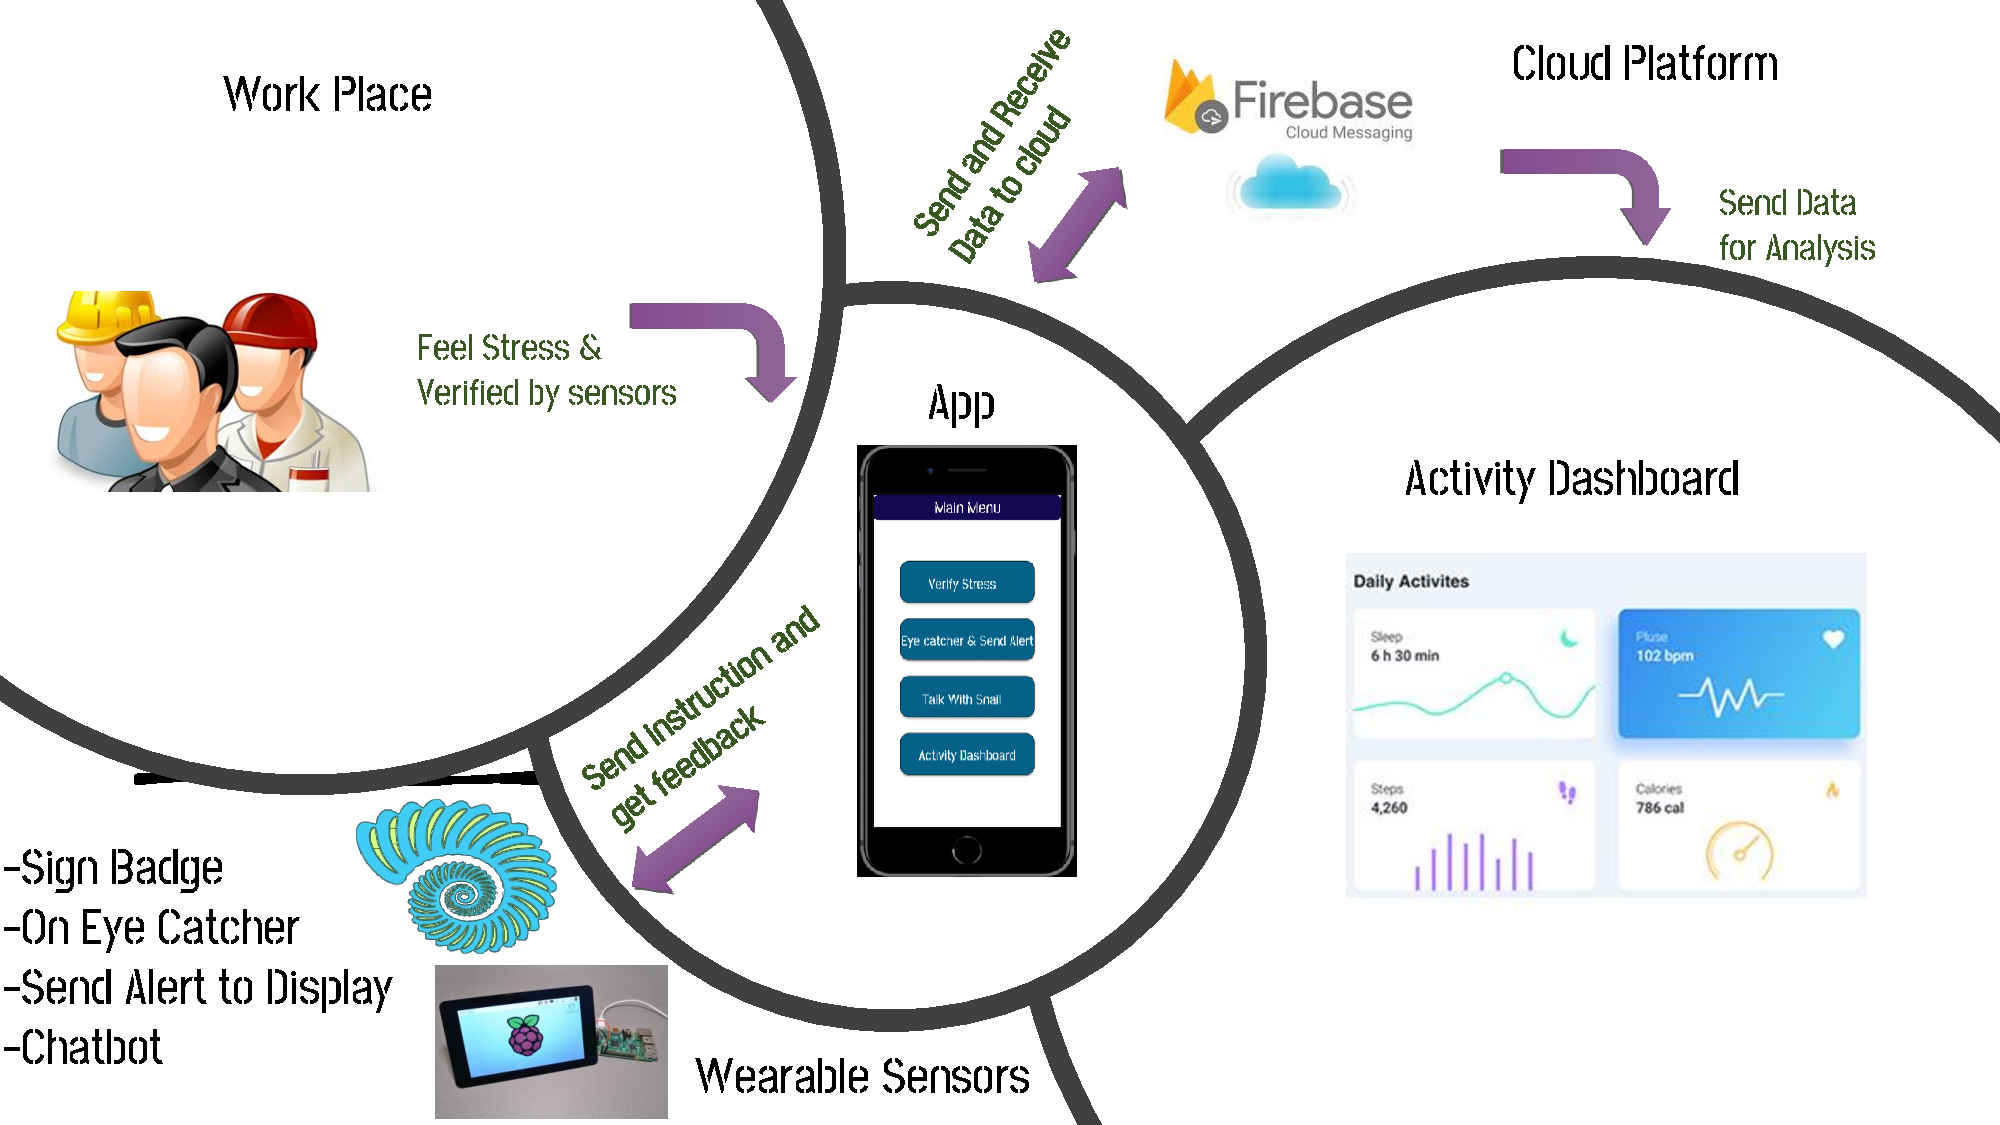
\includegraphics[width=1.0\linewidth]{chap4/image4/Overview.pdf}
  \caption[Schneckenhaus system overview ]{Schneckenhaus system overview\index{Hasnain}}
  \label{fig:overview_Stress}
\end{figure}
Schneckenhaus system combined with android app, multiple wearable sensors, IoT devices, physical eye-catcher, chatbot, activity dashboard. In figure :\ref{fig:overview_Stress} draw an ecosystem, how the system will work and will be the reaction and communication between components of the system. Let me explain the system working process. This system is suitable for the workplace environment and for people who have stress overflow.

In the workplace, the employee has lots of activity throughout the day. They do not always feel stressed. when they feel stressed my Schneckenhaus system area start from that point. I developed an android application as \acf{UI} for my system. This app main menu (See fig: \ref{fig:main_menu}) have the following four activity button which is connected with all components and tools of the system. 

\begin{enumerate}
    \item Verify stress
    \item Eye catcher and send Alert
    \item Talk with snail
    \item Activity Dashboard
\end{enumerate}

\begin{figure}[hbt!] 
  \centering
  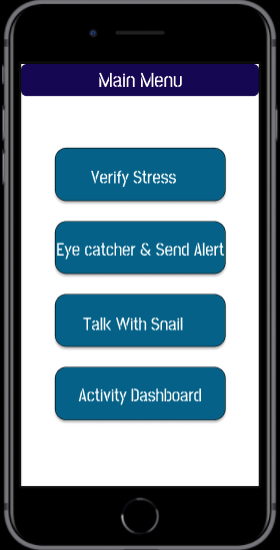
\includegraphics[width=0.4\linewidth]{chap4/image4/SC2.png}
  \caption[Schneckenhaus System UI app Main Menu ]{Schneckenhaus System UI app Main Menu\index{Hasnain}}
  \label{fig:main_menu}
\end{figure}

\subsubsection*{Verify stress}
In a stressed situation, the employee opens the Schneckenhaus app and press Verify stress activity button. The system will connect immediately to the two components of this activity. one is heart rate sensor via smartwatch another one is \acf{SpO2} for check the current heart rate and oxygen level of blood. this two components result Will verify user stress level with feelings. 
\subsubsection*{Eye catcher and send Alert}
when system recognized user is in stress app suggest to go for the next option which is an Eyecatcher and send an alert. This activity has three component. First one is a special sign badge, the user has to wear this badge on their shirt. the second one is Eyecatcher, it's a Schneckenhaus symbolic lightbox with two colour light green and blue. User can control the light via my Schneckenhaus app. Green light means no stress and blue light means stress overflowed which I found from persona analysis in chapter \ref{Persona Analysis Outcome}. then send customize massage or emoji to wireless display to inform concerns.
\subsubsection*{Talk with snail}
After acknowledging to the surrounding environment, the user needs to distress his stress. On this point, my system will suggest user Talk to Snail. Snail is the name of my chatbot. Snail name comes from the English name of  Schneckenhaus. In this system, Snail is the virtual assistant and trusted friend. In the back-end, it's connected with google Dialogflow API. This API use \acs{NLP} and \acs{AI} process conversion model. The snail will instruct user for doing some physical activity (e.g take five deep breath for 30 seconds) which will make use relax. Its also interact with the user-based conversation.
\subsubsection*{Activity Dashboard}
User, all activity throughout the system with the above mention activity will be recorded and send to the cloud server. This activity data use for the source of my system dashboard for visualization. When a user feels relax or does not have overflowed stress, they can check their activity. The user also can learn from his activity and take appropriate action if needed. This activity dashboard developed in React.js framework. React.js is one of the popular JavaScript frameworks to develop web-based visualization.

In the next section of this chapter, I will explain the Schneckenhaus system UI activity and components in details.

\section{Verify Stress}
\begin{figure}[hbt!] 
  \centering
  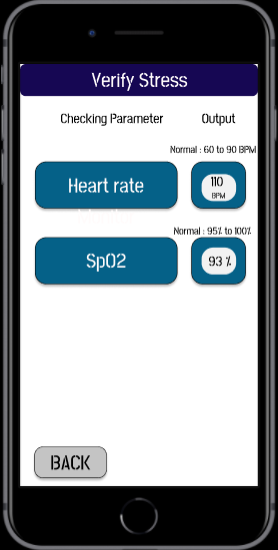
\includegraphics[width=0.4\linewidth]{chap4/image4/sensor.png}
  \caption[Verify Stress activity Component ]{Verify Stress activity Component \index{Hasnain}}
  \label{fig:Verify_Stress}
\end{figure}
In this activity, I designed and developed a system  to verify the psychophysiological signals monitoring stress during workplace and send data to cloud for analysis. 

In the workplace when you feel the stress they can immediately go to the app then press verify stress option. Figure: \ref{fig:Verify_Stress} shows the UI of Verify Stress Activity.The app will give two different types of health data from \acs{IoT} sensors.

\begin{itemize}
    \item 1. Heart rate sensor
    \item 2. \acf{SpO2} Sensor
\end{itemize}

In measuring health status, sensors and smartphones usually imply: collecting sensor data; providing user support through a display with the measured values; sharing information; ensuring low power devices, wear-ability, accuracy, durability and system reliability.

\subsection{Smart watch Heart rate sensor}
\begin{figure}[hbt!] 
  \centering
  \subbottom[Front view]{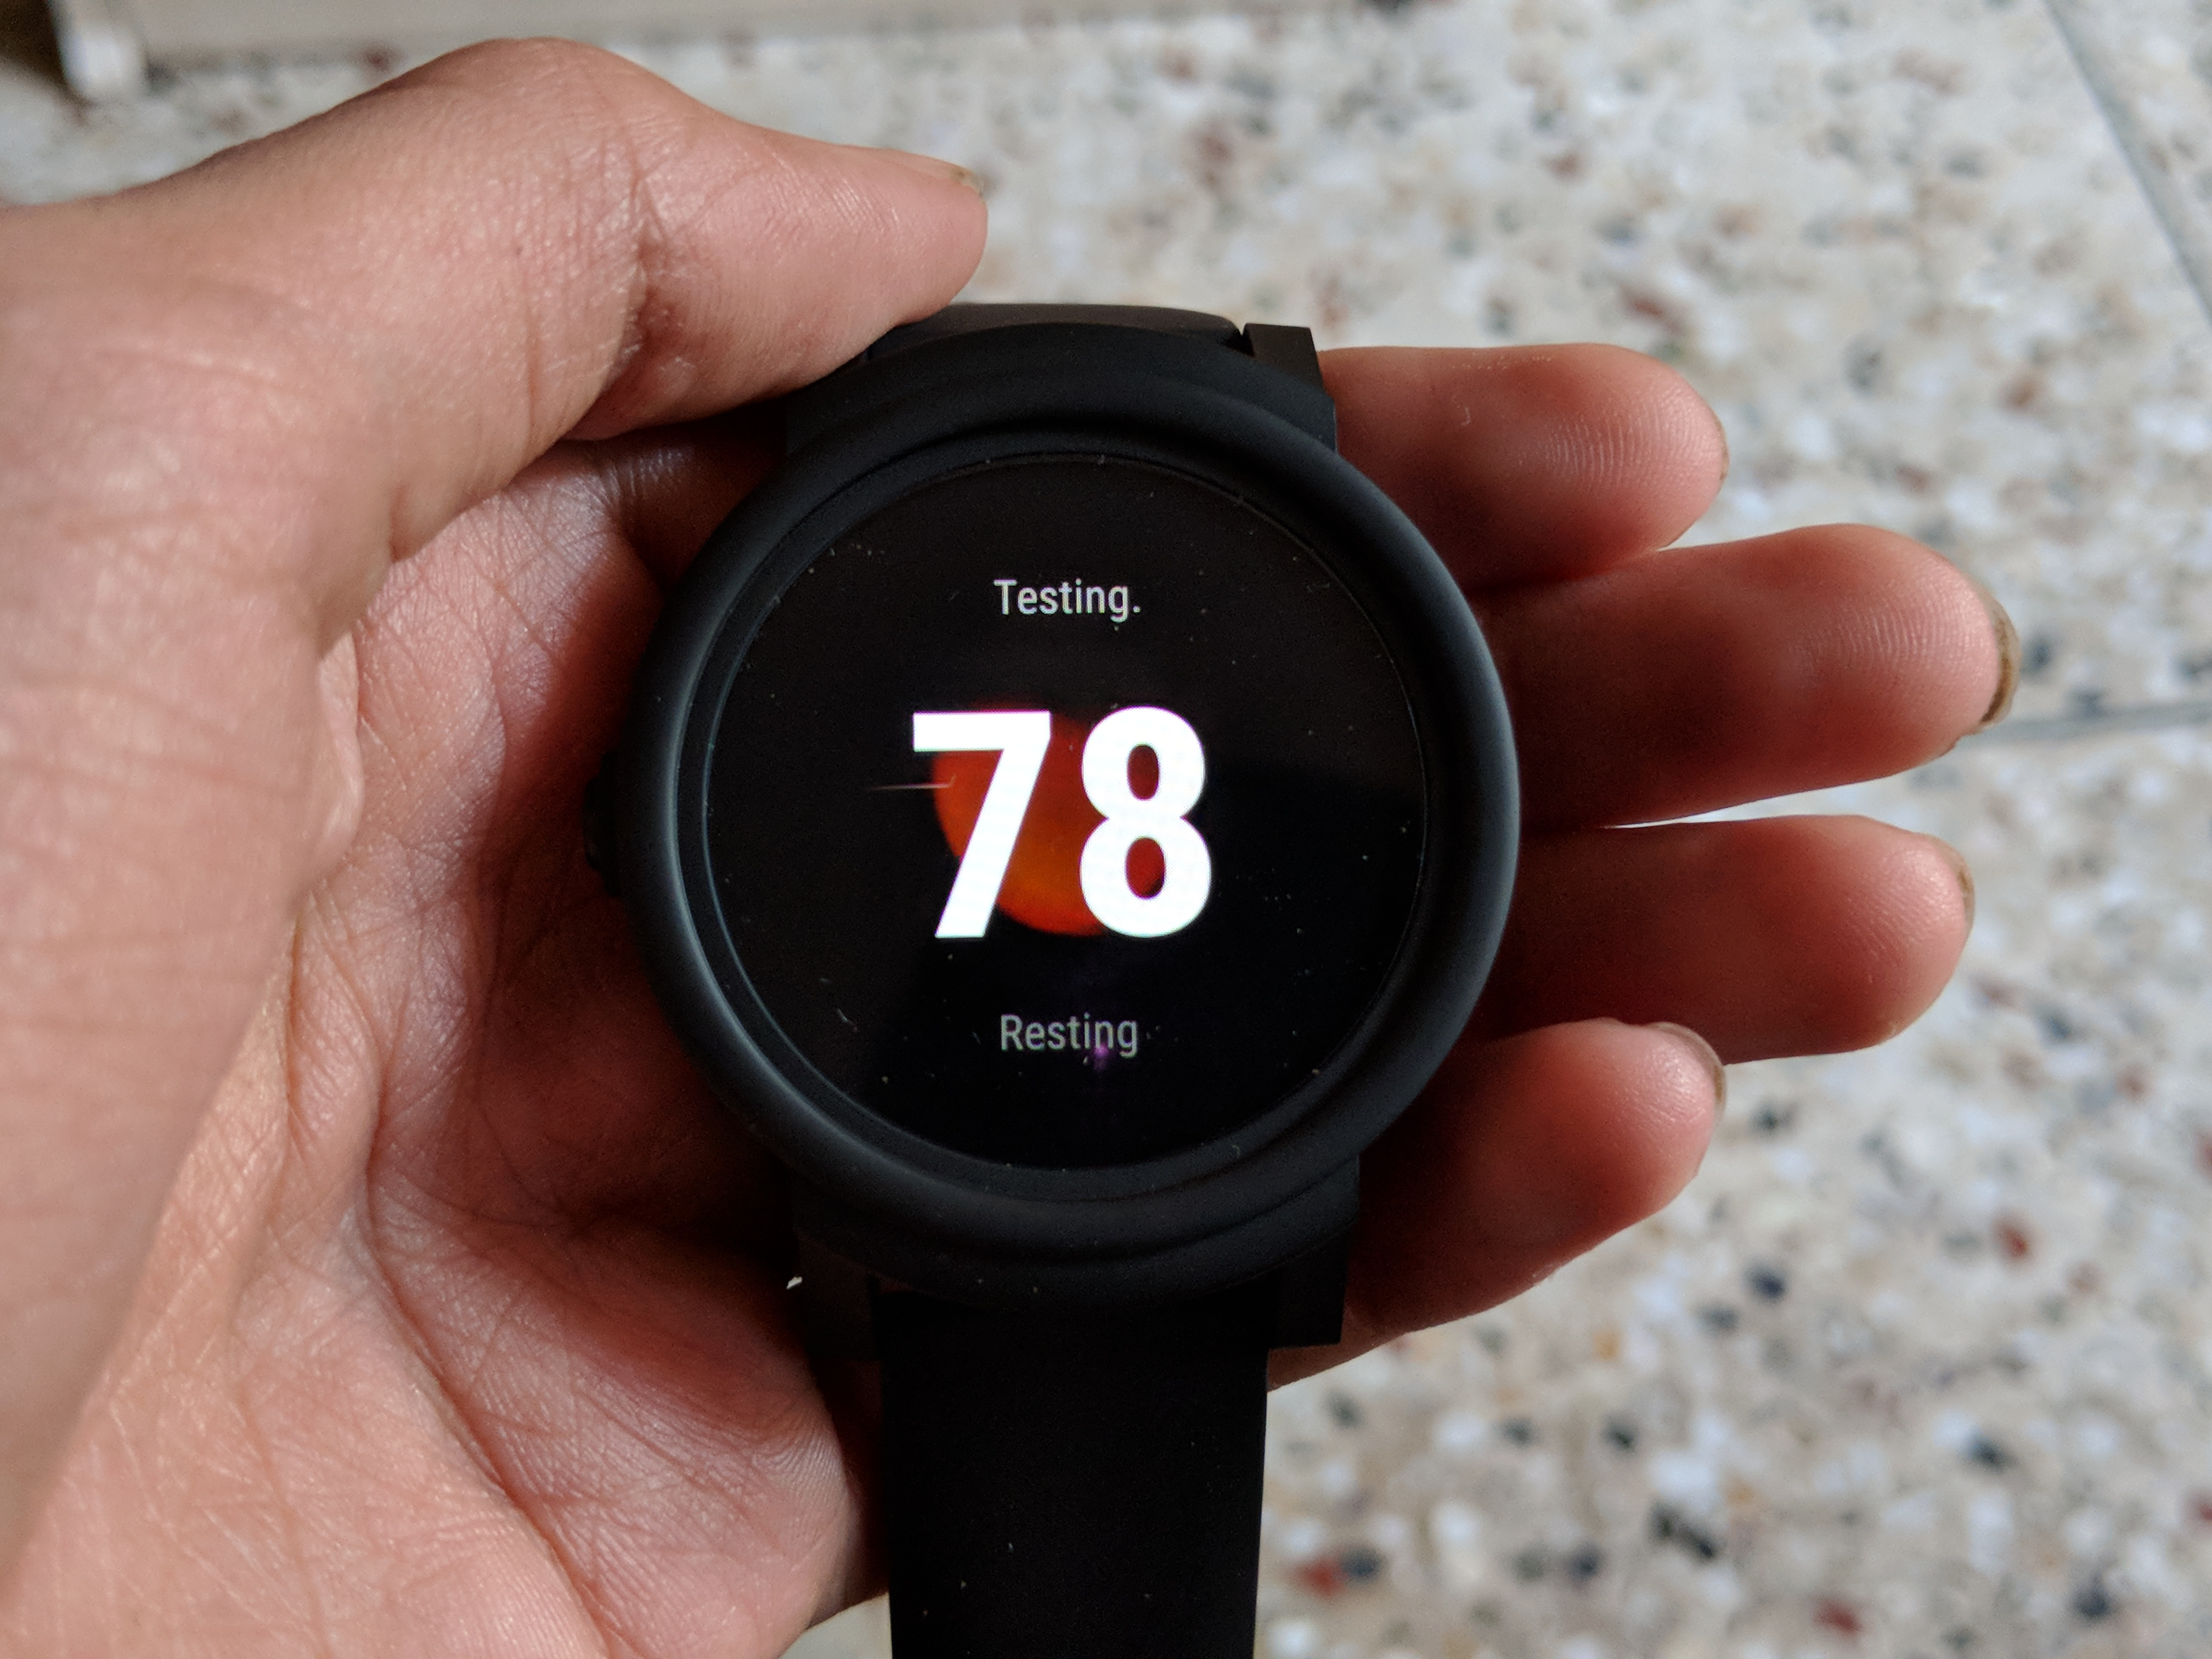
\includegraphics[width=0.45\textwidth]{chap4/image4/tikwatch.jpg}}\qquad
    \subbottom[Back side sensor view]{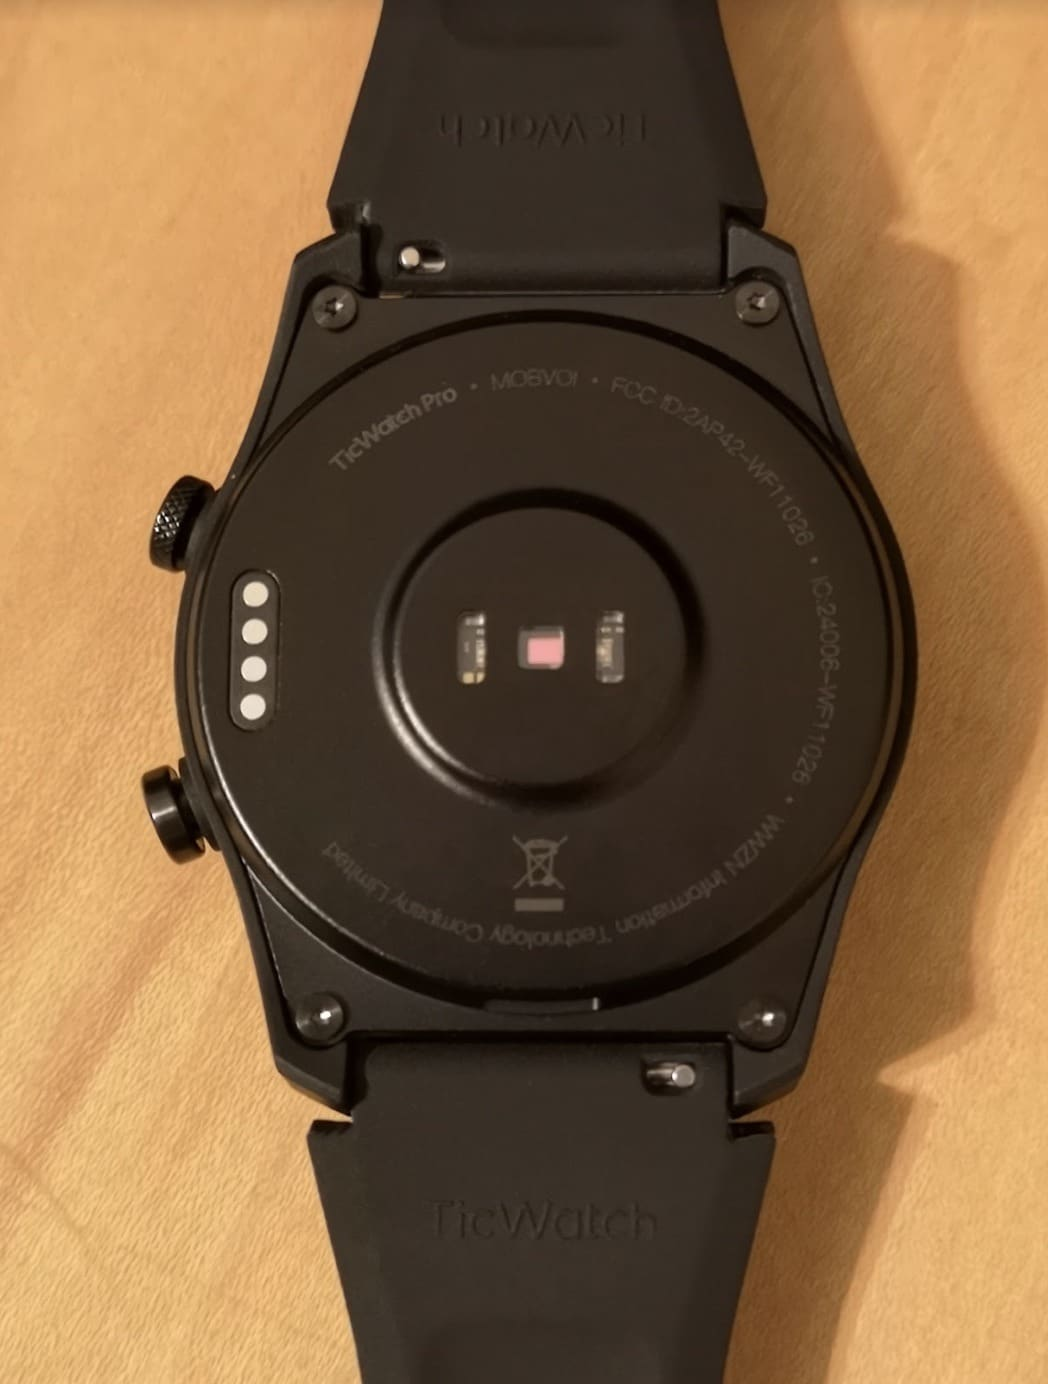
\includegraphics[width=0.26\textwidth]{chap4/image4/tikwatch1.jpg}}
  \caption[Ticwatch Smartwatch S2, Wear OS ]{Ticwatch Smartwatch S2, Wear OS\index{Hasnain}}
  \label{fig:Ticwatch}
\end{figure}
One of the main challenges is the design of a wearable, low-power, reliable and precise \acs{IoT} system. Commercial solutions also satisfy the criteria set out above.  One such solution is the fully wearable Ticwatch Smartwatch S2, Wear OS (shown in Fig.\ref{fig:Ticwatch}). The device has a Bluetooth module which allows communication with a suitable mobile application. This comes with no Google Fit API, as most commercial solutions do, and is thus programmable and customise able. Therefore, for real-time monitoring, further analytic, biofeedback, or integration with other educational services, there is possible to collect sensor data and store it in the Firebase database.

To maintain homeostasis, physical or mental imbalance induced by harmful stimuli can induce stress. The sympathetic nervous system is hyperactivated during chronic stress which causes physical, psychological, and behavioural abnormalities. There is currently no accepted standard for assessing stress. This analysis aimed to survey studies that provide a basis for choosing variation in the \acf{HR} as a measure of psychological stress.\citep{Kim2018StressLiterature}

User heart rate is changing from one minute to another. It depends on whether you stand or lie, move around or sit still, stressed or relaxed. Nonetheless, the restful heart rate continues to be steady every day. The usual heart rate resting range is between 60 and 90 beats per minute, anywhere. Over 90 is generally considered high.\citep{LeWine2011IncreasePublishing}
\subsection{\acf{SpO2}}
\acs{SpO2} stands for saturation of the peripheral capillary oxygen. It estimates how saturated the oxygen in your blood is. A safe, fit person usually sees a \acs{SpO2} ranging from 95\% to 100\%. Illness, altitude, heart disease, inhalation of smoke all have \acs{SpO2} effect.\citep{Sly2019ManagingBiostrap}
\begin{figure}[hbt!] 
  \centering
  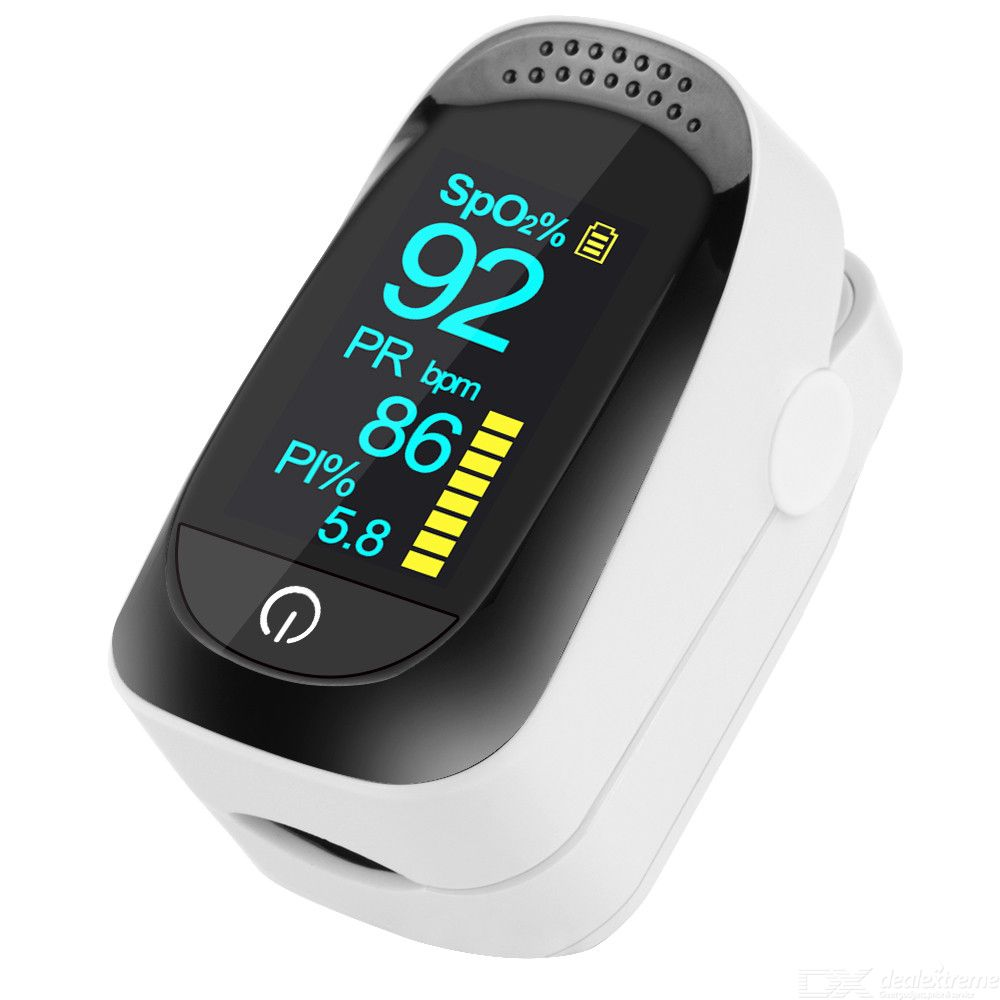
\includegraphics[width=0.5\linewidth]{chap4/image4/spo22.jpg}
  \caption[\acf{SpO2}]{\acf{SpO2}(source:\cite{Teleportz2019A2Shop}\index{Hasnain}}
  \label{fig:spo2}
\end{figure}
 Measure of \acs{SpO2} may not vary as much as user resting heart rate and HRV, but a sudden drop is often an indication of stress. Traditionally, athletes who train at higher altitudes track \acs{SpO2} to help make sure they get enough oxygen. This is an easy metric to track with the correct device along with the resting pulse.

\acs{SpO2} instant measurement device shown in figure:\ref{fig:spo2}. In this activity, I use this device for verifying the stress with personal feelings. And send data to the cloud for further analysis and visualization.

\section{Eye catcher and send Alert}
This activity is the part of Symbolic Representation for Others. Symbolic representation is a communicative activity that distinguishes human beings from other species and brings them together within cultures and other social groups. This section explores symbolic representation in our study, and restrict our development to symbolic representation in the context of external symbols used in contact with others.
\begin{figure}[hbt!] 
  \centering
  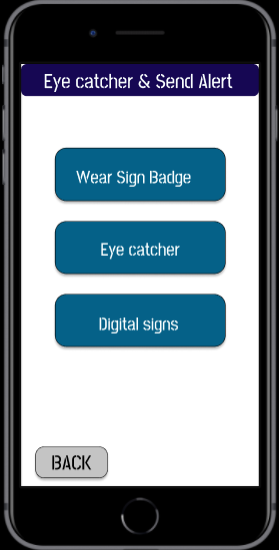
\includegraphics[width=0.4\linewidth]{chap4/image4/eye.png}
  \caption[Symbolic Representation for Others activity Component ]{Symbolic Representation for Others activity Component\index{Hasnain}}
  \label{fig:Sign}
\end{figure}
I used Three types of Symbolic representation for alert surrounding at work place.
\begin{itemize}
    \item Special Sign Badge
    \item Eyecatcher
    \item Digital signs to Wireless display
\end{itemize}

\subsection{Special Sign Badge}
In this activity, I use \textbf{Schneckenhaus} symbol badge as a metaphor of stressed condition. A stress status symbol is a visible perceived, external denotation of one's social position and perceived social status indicator.\citep{Cherrington1994OrganizationalBehavior} Many luxury goods are often considered status symbols. A status symbol is also a sociological term relating to how individuals and groups interact and interpret various cultural or stressed symbols, as part of social and sociological symbolic interactionism.
\begin{figure}[hbt!] 
  \centering
  
\includegraphics[width=0.4\linewidth]{chap4/image4/logo1.png}
  \caption[Schneckenhaus symbol sign badge ]{Schneckenhaus symbol sign badge\index{Hasnain}}
  \label{fig:Sign_badge}
\end{figure}
In this activity, I use special sign badge(see figure \ref{fig:Sign_badge} for acknowledging other collages about user current status. It should be previously circulated among the workplace from \acs{HR}.
\subsection{Eye catcher}
Based on dictionary Eye catcher means a thing that attracts attention. In our thesis, we use eye-catcher as a box (see figure \ref{fig:eye}). We made this box in our FAB lab and design with our Schneckenhaus symbol. Inside the box, we used two-colour LED, Green and Blue. This Led control by stress management app.  When the user has stressed condition too high, they should turn on the blue LED. When stress condition is a normal condition the switch back to green. 
\begin{figure}[hbt!] 
  \centering
  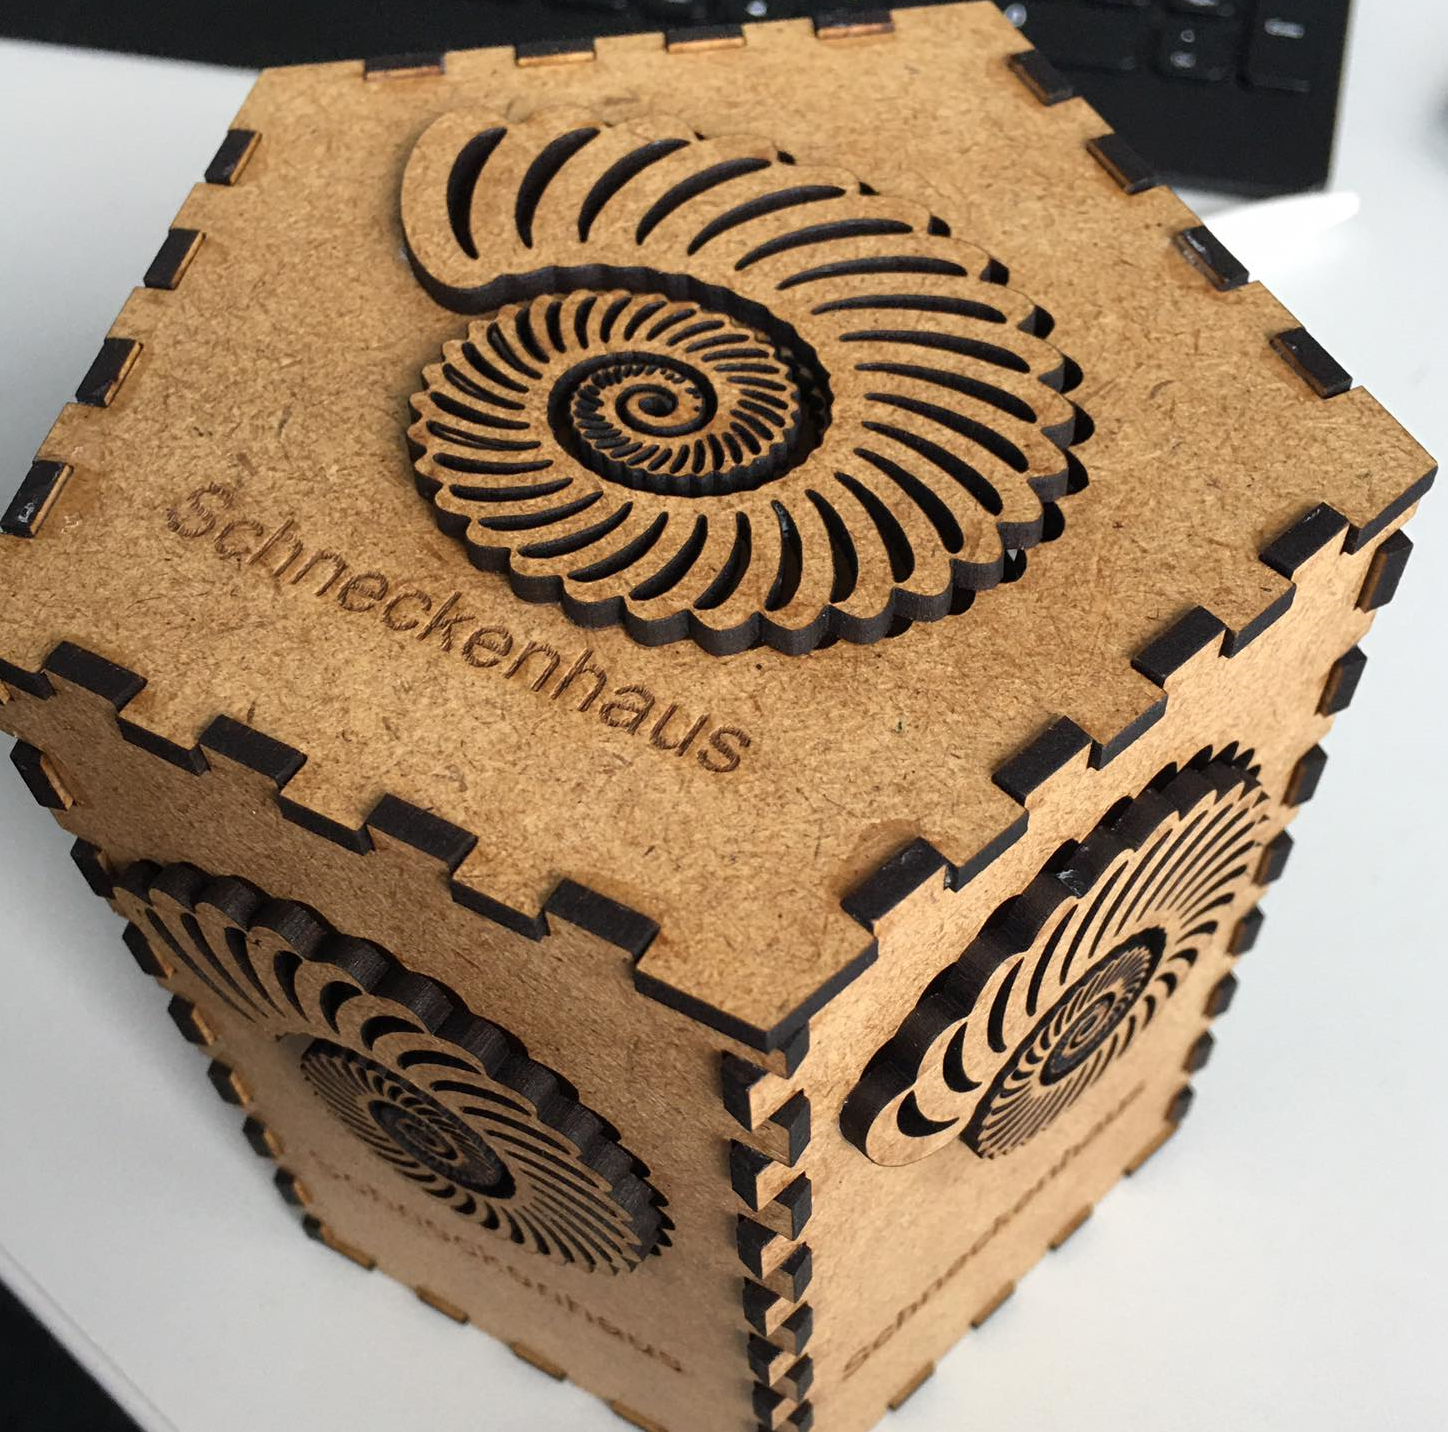
\includegraphics[width=0.5\linewidth]{chap4/image4/skn2.png}
  \caption[Eye catcher ]{Eye catcher\index{Hasnain}}
  \label{fig:eye}
\end{figure}
For communication with Schneckenhaus app with LED switching control we used NodeMCU device.

NodeMCU is an open-source \acs{IoT} platform which is low cost. Initially, it included firmware running on Espressif Systems ' ESP8266 Wi-Fi SoC, and hardware based on the ESP-12 module. Later, support was added for the 32-bit ESP32 MCU(see figure \ref{fig:node}.
\begin{figure}[hbt!] 
  \centering
  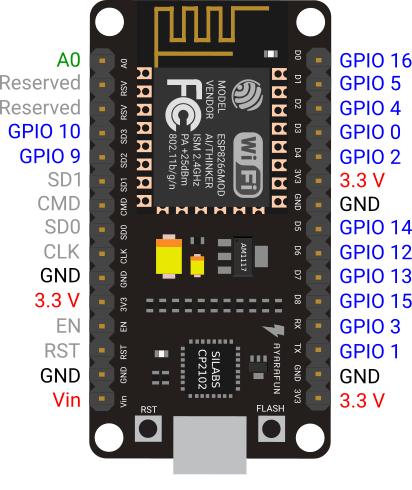
\includegraphics[width=0.5\linewidth]{chap4/image4/Node.png}
  \caption[NodeMCU with ESP8266 pinout ]{NodeMCU with ESP8266 pinout\index{Hasnain}}
  \label{fig:node}
\end{figure}
For writing code inside the NodeMCU used Arduino IDE. See below code. It explain how I wrote code to control LED through our Schneckenhaus app. I attached full code details in appendix. 

\begin{lstlisting}
// Read the first line of the request
  String req = client.readStringUntil('\r');
  Serial.println(req);
  client.flush();
  
  // Match the request
  int val;
  if (req.indexOf("/gpio/0") != -1)
    val = 0;
  else if (req.indexOf("/gpio/1") != -1)
    val = 1;
  else {
    Serial.println("invalid request");
    client.stop();
    return;
  }

  // Set GPI0 according to the request
  digitalWrite(D4, val);
  
  client.flush();

  // Prepare the response
  String s = "HTTP/1.1 200 OK\r\nContent-Type: text/html\r\n\r\n<!DOCTYPE HTML>\r\n<html>\r\nGPIO is now ";
  s += (val)?"high":"low";
  s += "</html>\n";

  // Send the response to the client
  client.print(s);
  delay(1);
  Serial.println("Client disonnected");

  // The client will actually be disconnected 
  // when the function returns and 'client' object is detroyed
}
\end{lstlisting}

\subsection{Digital signs to Wireless display}
\begin{figure}[hbt!] 
  \centering
  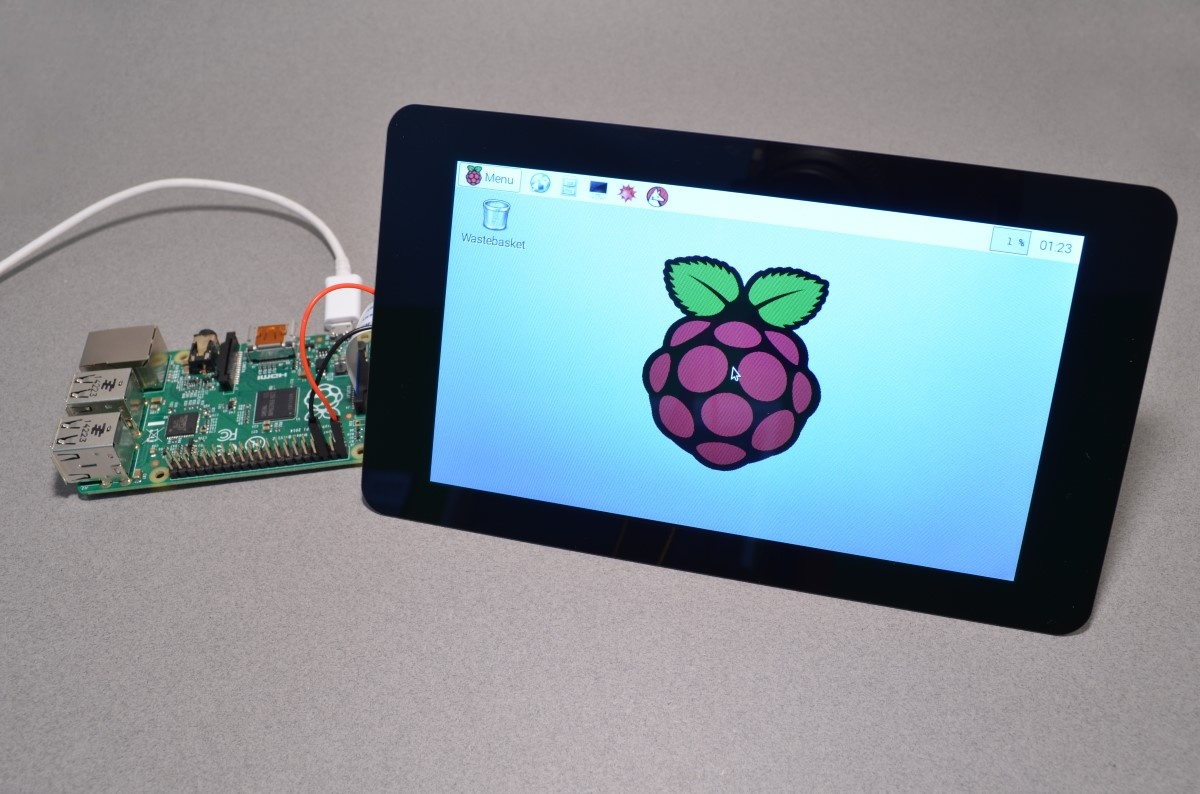
\includegraphics[width=0.5\linewidth]{chap4/image4/dipl.jpg}
  \caption[Raspberry PI Wireless display ]{Raspberry PI Wireless display\index{Hasnain}}
  \label{fig:PI_disp}
\end{figure}
For this activity, I use digital signage concept to make wireless display for send alert or massage to respective person in the work place.

The emergence and ongoing development of \acf{DS} systems give rise to an increasing number of such systems ' technological capabilities. While these technological capabilities have attracted considerable attention in computer science research, scarce studies are exploring their application and effect.  Marketing, and retailing in particular, represents an applied science which could benefit from \acf{DS}.  Some studies demonstrate in support of this assumption that the presence of \acs{DS} showing emotional content creates favourable shopping experiences and positively influences consumer behaviour.\citep{Bauer2018ResearchRetail}

Digital signs help people with Stress Overflowed to communicate better with their colleague and managers. Teams can use digital signs on their office walls to show special massages. Digital signage is an innovative medium of communication due to its always-on existence, allowing individuals to easily view and communicate with digital signs during the hustle and bustle of their busy days.

I need digital signage software to launch the digital signage on Raspberry PI. This software helps me to change my display screen and to manage the content. It is, however, a critical component of any successful strategy for digital signage. \acs{DIY} digital signs can be complicated and time-consuming to keep up-to-date without digital signage management software.

I use Screenly OSE in this activity for contents management. I will explain how to deploy the Screenly OSE software for open-source digital signage using balenaCloud. With balenaCloud, users can use the Public URL feature to manage their Screenly OSE powered digital signs from anywhere with an internet connection. This remote management is a game-changer for stress management in the workplace, as it is.

\section{Interactive Chatbot}
A chatbot is a \acf{AI} program that simulates interactive human conversation using key pre-calculated user phrases and auditory or text-based signals. Chatbots are often used for basic customer service and marketing systems which frequent hubs of social networking and \acf{IM} customers. They too are often included in operating systems as intelligent virtual assistants.
\begin{figure}[hbt!] 
  \centering
  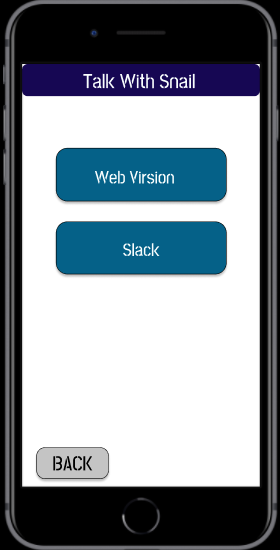
\includegraphics[width=0.4\linewidth]{chap4/image4/chat.png}
  \caption[Interactive Chatbot (Snail) activity Component ]{Interactive Chatbot (Snail) activity Component\index{Hasnain}}
  \label{fig:chat}
\end{figure}

Also known as a chatbot is a \acf{ACE}, chat robot, talk bot, chatterbot, or chatterbox. In our thesis, we used chatbot as trusted in the workplace. In figure \ref{fig:chat} shows the process diagram of chatbot activity. The chatbot will interactively talk with the user and suggest some activity for relaxation. 

I used two platforms to make this bot, one is web-based using React.\acs{js} and Dialogflow \acs{API}. Another one is Slack platform which most commonly used for corporate communication in the workplace. I integrate slack with Dialogflow \acs{API}.In figure: \ref{fig:Slackchat} shows the Slack Chatbot (Snail) Interface.

\begin{figure}[hbt!] 
  \centering
  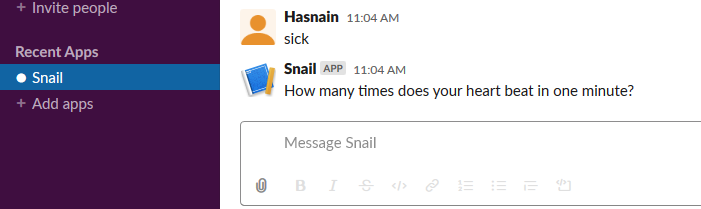
\includegraphics[width=1.0\linewidth]{chap4/image4/slack_chat.png}
  \caption[Slack Chatbot(Snail) Interface ]{Slack Chatbot(Snail) Interface\index{Hasnain}}
  \label{fig:Slackchat}
\end{figure}

Dialogflow is a Google-owned human-computer interaction technology company based on conversations in the natural language. The company is best known for creating the Assistant, a virtual mobile buddy for Android, iOS, and Windows Phone that performs tasks and answers user questions in a natural language.\citep{Zax2012TheSolved} Speaktoit has developed a natural language processing system that integrates the context of interaction such as dialogue history, location, and user preferences. This is the main reason we chose Dialogflow back-end for our system.

Use Dialogflow API A prototype chatbot called \textbf{Snail} has been developed to make access to a self-help library simpler for a more immersive user journey. The library of self-help consists of such categories as abuse of anxiety, depression, obesity, and alcohol/drug. That category contains numerous data files which contain information about each category. To find the information they are searching for, the user is expected to click in the various categories. The chatbot was designed to provide a more engaging way to lead the user to workplace stress relief and ask them what areas they would like information about.

In this activity, we build a system employs chatbots to conduct a conversation with individuals to derive a measure of stress using a Sense of Coherence conversation. The outputs of this conversation then drive an analysis dashboard which selects and administers an intervention intending to reduce measured stress. The conversation and Sense of Coherence conversation that we develop are capable of measuring stress and can be used by the analysis dashboard to successfully select appropriate support actions.

\section{Stress Analytic Dashboard}
In the firebase cloud database, I stored activity metadata about the sensors and chatbot interaction, which is not understandable, which annotations are wrong. Visualize the sensor and chatbot interaction data and the annotated information with it I used \acf{js} based visualization tool, which helps users. Therefore, the user can understand, when and what was the stress level during the working time. So the user can take appropriate measures when stress overflow and monitor users activity. The activity dashboard feature of our system for visualizing data is shown by the following figure.
\begin{figure}[hbt!] 
  \centering
  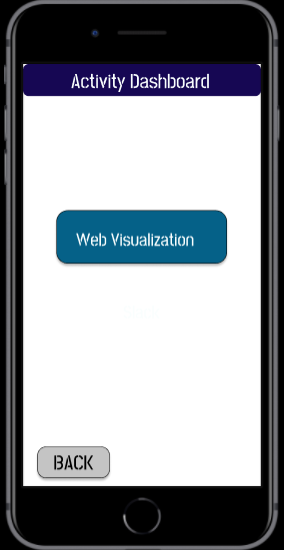
\includegraphics[width=0.4\linewidth]{chap4/image4/dashboard.png}
  \caption[Stress Analytics Dashboard Activity ]{Stress Analytic Dashboard Activity\index{Hasnain}}
  \label{fig:dashboard}
\end{figure}
Activity Analysis dashboards can be used for a variety of purposes, including strategy analysis and execution, performance reviews, performance improvement, data comprehension, and scope opportunity. But why is the format better than other visualizations of the data? Here are three main benefits of the Stress Management dashboards:
\subsubsection*{Access \& Understand Data:}
An Activity dashboard summarizes and visualizes data in a way that makes it easy to understand what’s important and what needs immediate attention. It shows personal performance at a glance. From there, users can make quick analyses and take action with confidence, backed by data. 
\subsubsection*{Predict Trends:}
Providing a high-level, graphic view of a facility’s numbers helps the empowerment spot trends. A dashboard shows if a \acs{KPI} is tracking above or below its benchmark over time in the workplace. User can make predictions and quickly adjust the strategy or goals when needed.
\subsubsection*{Prioritize:}
Another benefit of dashboards in Activity Analytic is they display individuals most essential data. User can drill down into any \acs{KPI} to get more information, but everything is rolled up into high-level goals. This helps establish priorities because you can see how the minute data affects the larger goals.

Activity Analytics Dashboard offers you a comprehensive view of the data. User needs to focus on areas that need immediate attention while filtering out distractions.

\begin{figure}[hbt!] 
  \centering
  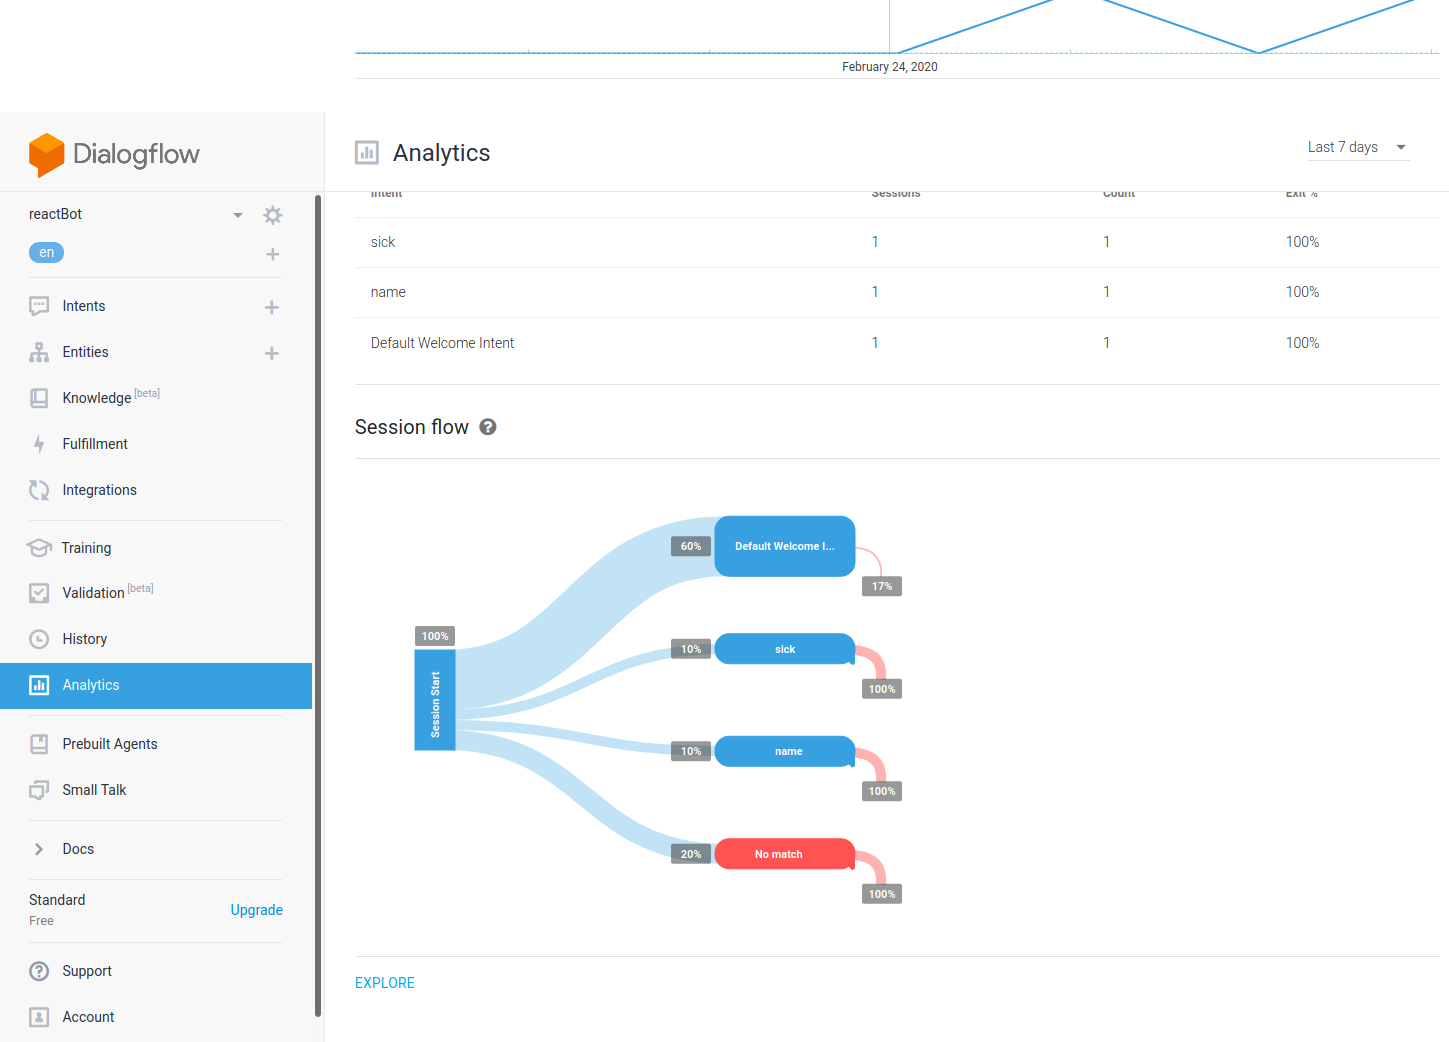
\includegraphics[width=1.0\linewidth]{chap4/image4/flow2.png}
  \caption[Dialogflow chatbot session activity visualization ]{Dialogflow chatbot session activity visualization\index{Hasnain}}
  \label{fig:flow2}
\end{figure}

In this activity, I develop an Activity Analytics Dashboard using react.js and Dialogflow API to analyze the activity of Stress Overflowed people in the workplace.  In figure \ref{fig:flow2} shows the one session chatbot activity visualization at Dialogflow.

To sum up; this chapter has discussed the development of the system for this study. I have addressed the process, activity and development tools. Afterwards, the next chapter of the thesis will discuss the experiment and result that I have gotten from the prototype experiment by the participant.



    \chapter{Experiment and Result}

\textbf{In an ideal world, you should have two kind of evaluations.  The first is against some ground truth (perhaps a random model?).  The second kind of evaluation is against other people's work (accuracy, speed, etc.).  Any dimension which is of interest, should be evaluated.  Evaluation should be statistically sound. }

\Blindtext
\section{Participants}
\section{Duration}
\section{Qualitative Feedback}
    \chapter{Discussion}
\textbf{This section should have a summary of the whole project.  The original aims and objective and whether these have been met should be discussed. It should include a section with a critique and a list of limitations of your proposed solutions.  Future work should be described, and this should not be marginal or silly (e.g.\ add machine learning models).  It is always good to end on a positive note (i.e.\ `Final Remarks').}



    \chapter{Future Work}
\textbf{This section should have a summary of the whole project.  The original aims and objective and whether these have been met should be discussed. It should include a section with a critique and a list of limitations of your proposed solutions.  Future work should be described, and this should not be marginal or silly (e.g.\ add machine learning models).  It is always good to end on a positive note (i.e.\ `Final Remarks').}


    \chapter{Conclusions}
\textbf{This section should have a summary of the whole project.  The original aims and objective and whether these have been met should be discussed. It should include a section with a critique and a list of limitations of your proposed solutions.  Future work should be described, and this should not be marginal or silly (e.g.\ add machine learning models).  It is always good to end on a positive note (i.e.\ `Final Remarks').}


 
6. Concluding Remarks 
This  chapter  presents  the  conclusions  of  our  research  by  encompassing  a  summary  of  the 
most important results from the whole thesis. The conclusions made are linked to our analysis 
and are also in line with our research aim which is to have a clear understanding of what 
causes stress at a multinational company such as Volvo trucks AB Umeå and how Stress by 
the employees as well as the company’s management are managed or handled.    
 
Based on the combination of our empirical study done at Volvo Trucks AB Umeå and our 
literature review we have reached the following conclusions. Our empirical data is reliable to 
the extent that it helped us in attaining our aim which was to find the causes and management 
of stress by both the employees and managers at Volvo Trucks AB Umeå. Our research by 
considering  Volvo Trucks  AB Umeå personnel  made it even  clearer to  what  the causes of 
stress  are  in  an  actual  company  and  how  the  employee  as  well  as  management  deals  with 
them. This gave us a clear guidance towards answering our research question. The theoretical 
framework assisted us to understand what causes stress and how it can be managed. Where as 
the  empirical  findings  allowed  us  to  see  this  from  Volvo  Trucks  AB  Umeå  employees’ 
perspectives and the analysis created a link between the theories and the empirical findings 
and summarized what the causes and management mechanisms of stress at a manufacturing 
multinational company such as Volvo Trucks AB Umeå are.   
 
6.1 Conclusions            
Our research using qualitative methods to understand the causes of stress at the work place 
particularly at Volvo Trucks AB Umeå and also observe the management mechanisms applied 
by both the employees and the management at Volvo Trucks AB, Umeå can be concluded by 
our findings and analysis of our results are summarized as follows. 
After conducting this research we can conclude that regardless of the employees’ job level, 
position or belongings of department, employees at Volvo trucks AB Umeå do feel stressed 
like other companies’ employees do. Employees feel stress because of various factors, mainly 
on job and off job reasons. But not all the reasons are directly linked to the issues that create 
stress at the workplace. We think that the stress level among employees at Volvo trucks AB 
Umeå is normal and it is not more than the stress that people feel outside the organization. 
With regards to theories and information collected from the respondents during interviews, 
we come up with three main conclusions.  
 
Conclusion 1: causes of stress 
We wanted to see the main causes of stress at Volvo Trucks AB Umeå. So we found several 
reasons why employees feel stressed at the workplace, the reasons mainly were inability to 
manage  time,  work  overload  and noise  as  the  main  stressors  at  the  workplace.  But  it  is 
necessary  to  say  that  noise  is  subjective  only  to  our  study  as  we  did  our  case  study  on  a 
manufacturing  company  and  the  conclusion  that  noise  is  the  main  causes  of  stress  in  the 
workplace might not be valid beyond an industry that is of manufacturing. Work overload is 
also another main stressor because it puts the employee under pressure to perform too many 
tasks under limited time.  
 
As Volvo Trucks AB Umeå is a manufacturing company we were able to conclude that in a 
manufacturing  multinational  company  where  the  physical  environment  can  be  chaotic  and 
noisy, this situation can be the cause of stress. The conclusion that can be reached from the 58 
 
theories in relation to our purpose is that the workplace causes of stress are work overload, 
poor  working  conditions  such  as  overcrowded  working  conditions  and  noise.  From  our 
analysis we are also able to conclude that the environmental factors of stress are not salient in 
a  multinational  manufacturing  company  such  as  Volvo  Trucks  AB  Umeå  where  the 
employees  were  focused  on  the  internal  factors  of  stress  rather  than  the  external.    Stress 
factors are not always stable, consistent and similar to a group of occupations. It varies from 
environment to environment, work to work or situation to situation, 
Conclusion 2: Steps towards stress management 
We  also  add  to  our  findings  regarding  the  employees  stress  coping  styles  and  steps  that 
employees at Volvo Trucks AB Umeå seek out to their close relatives, friends and families for 
support and consultation. Sharing of feelings and emotions contribute to relieve stress  also 
provide  them  to  enjoy  from  their  professional  life  and  personal  life.  Being  able  to  share 
feelings with peers and families gives different perspective about the proper way to tackle a 
problem  besides  having  a  sense  of  companionship  leads  to  comfortable  workplace. 
Employees  mostly  use  these  tactics  during  the  periods  in  which  they  feel  stress.  However 
stress reduction depends on how the employees manage their time effectively and also how 
the  managers  make  the  workplace  stress  free.  We  also  conclude  that  stress  is  highly  self-
controllable and those employees have the ability to control their feelings and manage their 
stress and for the rest they can refer to the facilities that they are provided by the management. 
Lastly  we  would  like  to  conclude  that  sharing  values  concerning  ambition  level  is  vital  in 
order to experience a reduced stress level. In some instances the employees stress level will be 
affected if they do not know anything about their fellows or close colleagues who works in a 
team. It makes them to be afraid if their ambition level doesn’t match. Therefore it is vital to 
as much as possible to get to know each other’s better and share values and ambition level; 
this will thus affect the stress level and can help in stress reduction.  
 
Conclusion 3: Management of stress  
Lastly  we  add  to  this  conclusion  our  findings  regarding  the  stress  management  of  Volvo 
Trucks AB Umeå. We see that Volvo Trucks AB Umeå has provided a safe workplace for the 
employees.  It  obtained  an  international  award  because  of  having  a  safe  workplace.  Volvo 
trucks AB Umeå has provided medical health center for the treatment of employees stress. 
Employees have freedom to meet the therapist and psychologist as a reason of improving their 
self-esteem and assertiveness. Volvo trucks AB Umeå has also made free time activities and 
various sport facilities for the employees. We think that it is an effective way to support its 
employees in reducing their stress level.  
 
We have also found out from the employees opinion who contributed to this study that stress 
at  the  workplace  is  manageable  but  a  combination  of  both  family  and  work  stressors  are 
highly negative. What we found from the employees open-ended questions is that sometimes 
stress at a certain extent affects positively to their work performance. It makes the employees 
to focus on time management and provide them to render their on job and off job activities 
adequately.  
 
Employee’s stress can be managed by proper time management, seeking help from Human 
Resource Management. Emotion focused strategies like leisure activities, companionship and 
exercise can also be used to relieve stress. Management of a company  also plays an important role in evaluating and managing the stress level of employees at the workplace and should  
use different methods to minimize the stress such as conducting training courses to assist the 
employee’s skills, providing better working environment and making sure that the employees 
get proper guidance and consultation when it’s needed.  
 
To  some  up;  while  many  employees  struggle  with  stress,  in  worst  cases  it  leads  to 
uncertainties and severe impairments  on their health and performance.  The main situations 
that  generate  stress  are  likely  uncontrollable,  unpredictable,  and  are  not  known.  But 
alternatively there are several resources available like personal awareness in coping skills. For 
example:  time  management,  assertiveness,  ways  to  higher  up  self-confidence  and  so  on. 
Management can also utilize some resources for reducing the stress level of the employees by 
investing in training programs, work infrastructure, improving the efficiencies in management 
and employment practices and also trying some other ways which is profitable in organizing 
the work. 


Conclusion
In this thesis, an in-depth literature study was made as a support to two separate experimental studies. In the first experimental study, different stress measures derived using ECG were investigated and compared among each other.  The purpose was primarily to see if they show significant changes in stress load during a period of recovery, but also to compare them during this period. Forthe second experimental study, a real-time solution was created to investigate two respiratory components in an ECG-signal. This was done by monitoringthe two respiratory components during a controlled breathing exercise.  Thepurpose was to find out which one of these followed the breathing pattern themost, and therefore, would be most suitable for biofeedback. This was done bythe use of time and frequency domain algorithms.The first experimental study showed promising results for the stress mea-sures, where all stress measures detected a significant decrease ofstress loadduring a period of recovery. Which could indicate that all measurescould po-tentially work as parameter to identify stress. The most significant decrease wasgiven by the LF/HF ratio, which was taken from the frequency domain. How-ever, more steady decrease was shown for the RMSSD and heart rate signal.Thesuggested stress measure for further use was the LF/HF ratio. However, a stressmeasure based on the frequency domain of the signal would be problematic forreal-time measurements, thus, RMSSD and heart rate were implemented to thesecond study.By analyzing the plain signals, both respiratory components in the secondexperimental study followed the breathing pattern, more of less. They both hada specific feature which made it problematic for the algorithms to identify thecorrect amount of breaths. Compared to the heart rate signal, the R-peak am-plitude signal had a more uneven appearance with more noise. A feature whichwas present for the heart rate signal, that could not be seen for the R-peakamplitude signal, was baseline variations of the signal. During ECG measure-ments, the R-peak amplitude varies around zero, since the values represents thedifferences between R-peak amplitudes. The heart rate on the other hand maydiffer during the measurements due to varying heart rate. Both these signalappearances were also seen in the frequency analysis.Combining the algorithms and the frequency analysis, the heart rate signalfollowed the breathing pattern more accurately in comparison to the R-peakamplitude.With today’s stressful environment with increasing numbers ofstress-relateddiseases, it would be very interesting to implement these stress measures in awearable device. This would allow people to keep track of their stress, to beable to gain more knowledge and learn how to control it. Which hopefully couldbring a more healthy life to many stressful individuals.

    \appendix
        \chapter{Media Content}

If the dissertation has a DVD or pendrive attached to it, you will need a section which explains what is on the media (structure, files, data, etc.).  This could be a table with filename and description.

\blindtext
     % these are just test names as I didn't know what you'd want
        \chapter{Installation Instructions}
    
        \chapter{User Manual}

 

{\backmatter
    % Bibliography
    \if@openright\cleardoublepage\else\clearpage\fi
    \bibliographystyle{um-plainnat} %% specific plainnat does not show url for articles
    {\footnotesize\bibliography{references}}
	\printindex
}

\end{document}

%%% The End %%%